\subsection{Question 1}
\label{sec:study-question1}

\begin{center}{\it Which face has a larger nose?}\end{center}

\begin{figure}[h]
\centering
\begin{subfigure}{0.4\textwidth}
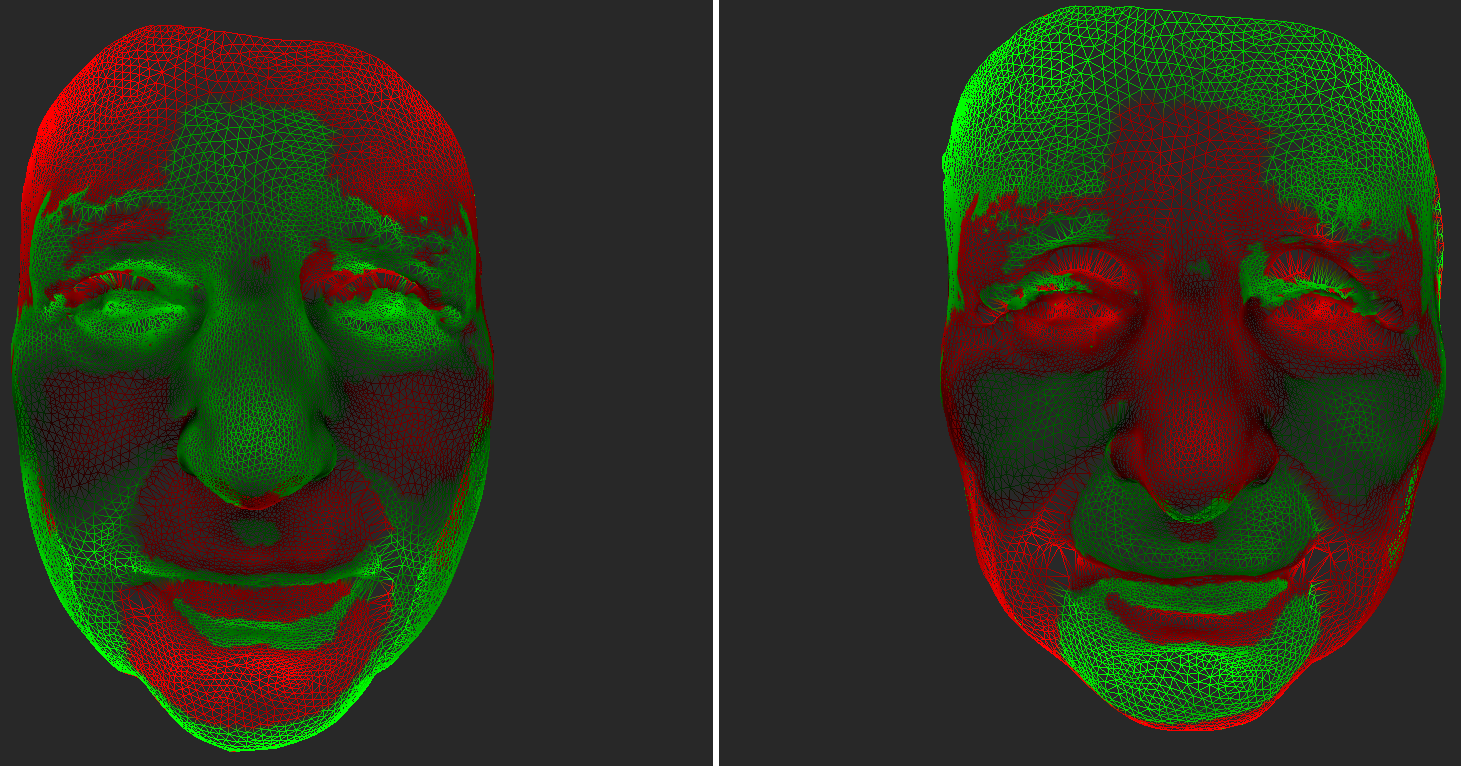
\includegraphics[width=\textwidth]{./screenshots/pair2.PNG}
\caption{}
\label{fig:0-2}
\end{subfigure}
\quad
\begin{subfigure}{0.4\textwidth}
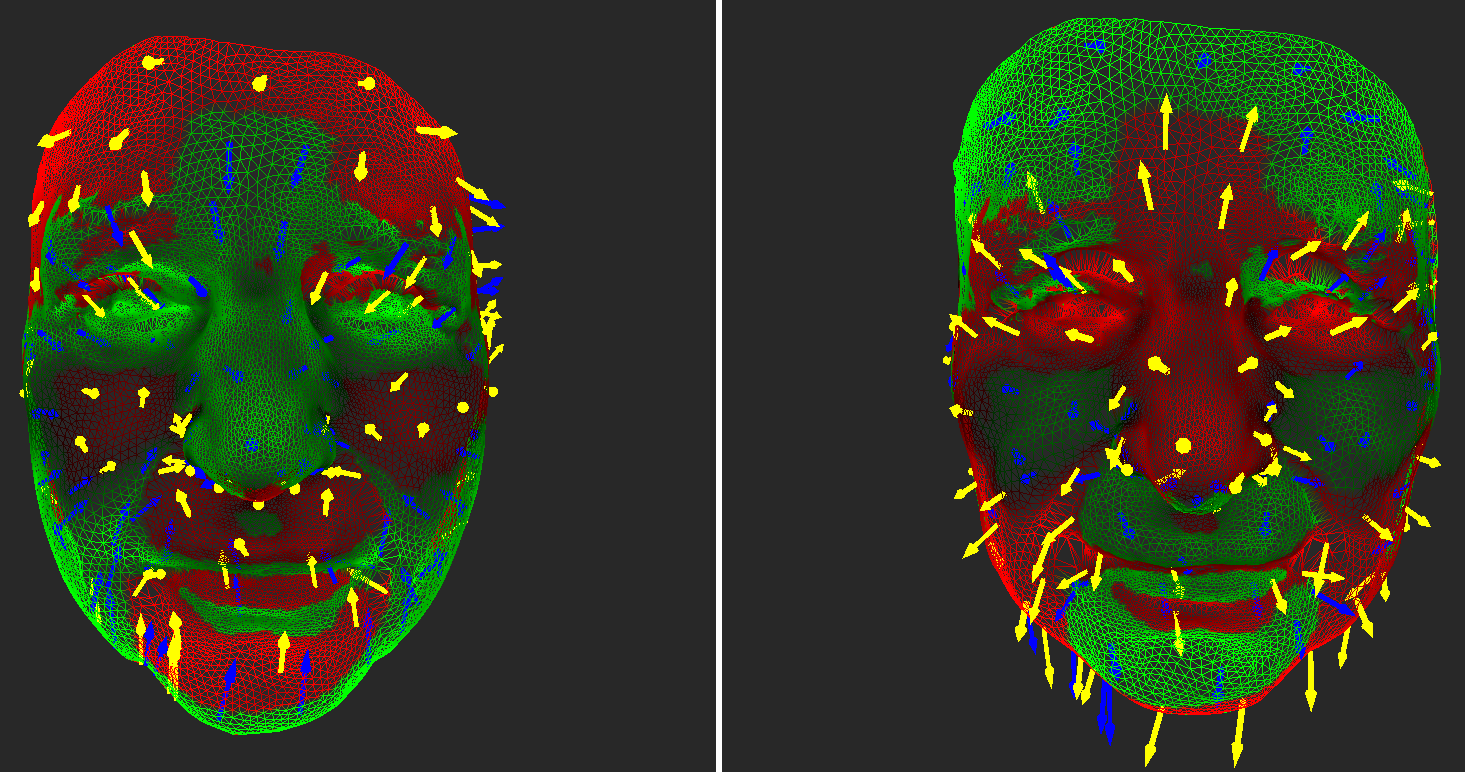
\includegraphics[width=\textwidth]{./screenshots/pair4.PNG}
\caption{}
\label{fig:0-4}
\end{subfigure}

\begin{subfigure}{0.4\textwidth}
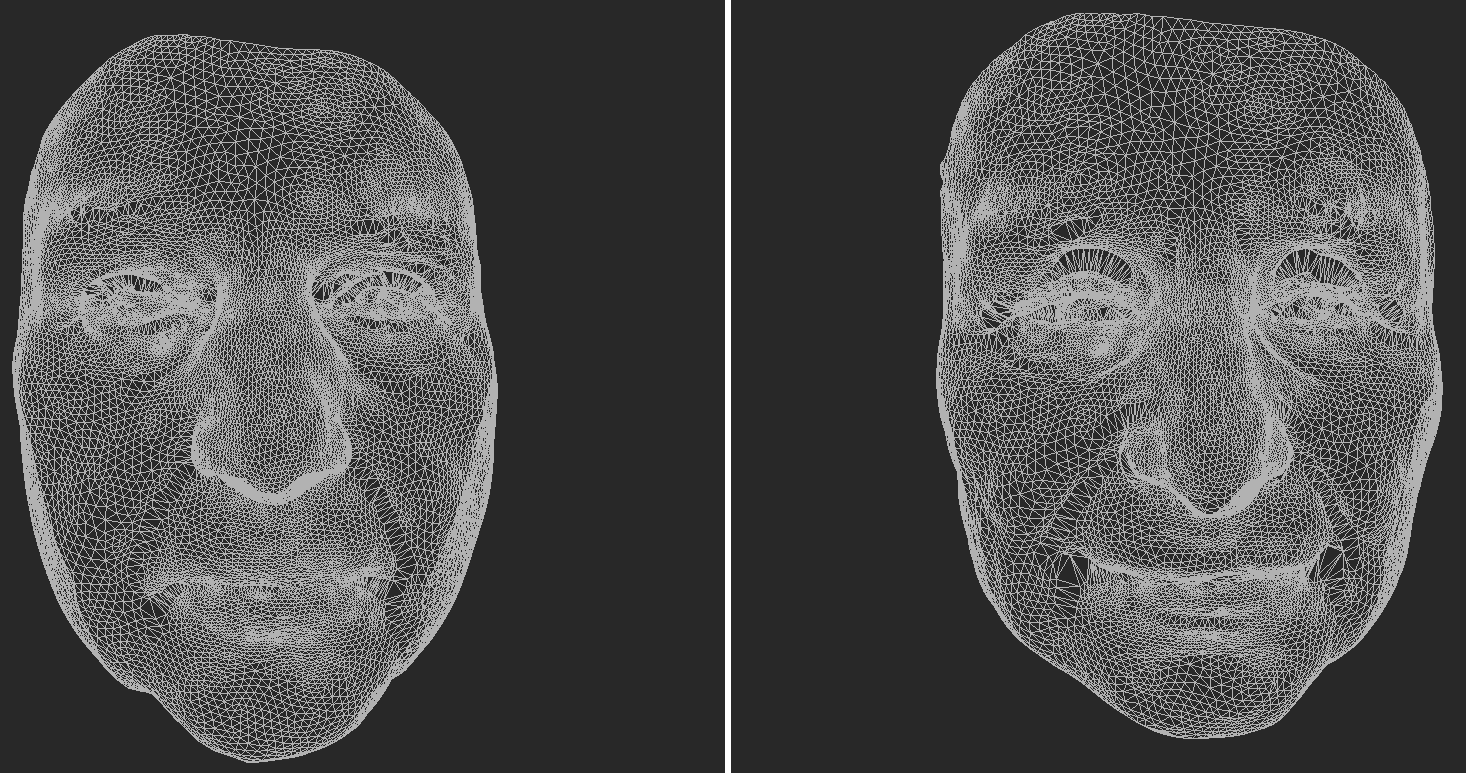
\includegraphics[width=\textwidth]{./screenshots/pair1.PNG}
\caption{}
\label{fig:0-1}
\end{subfigure}
\quad
\begin{subfigure}{0.4\textwidth}
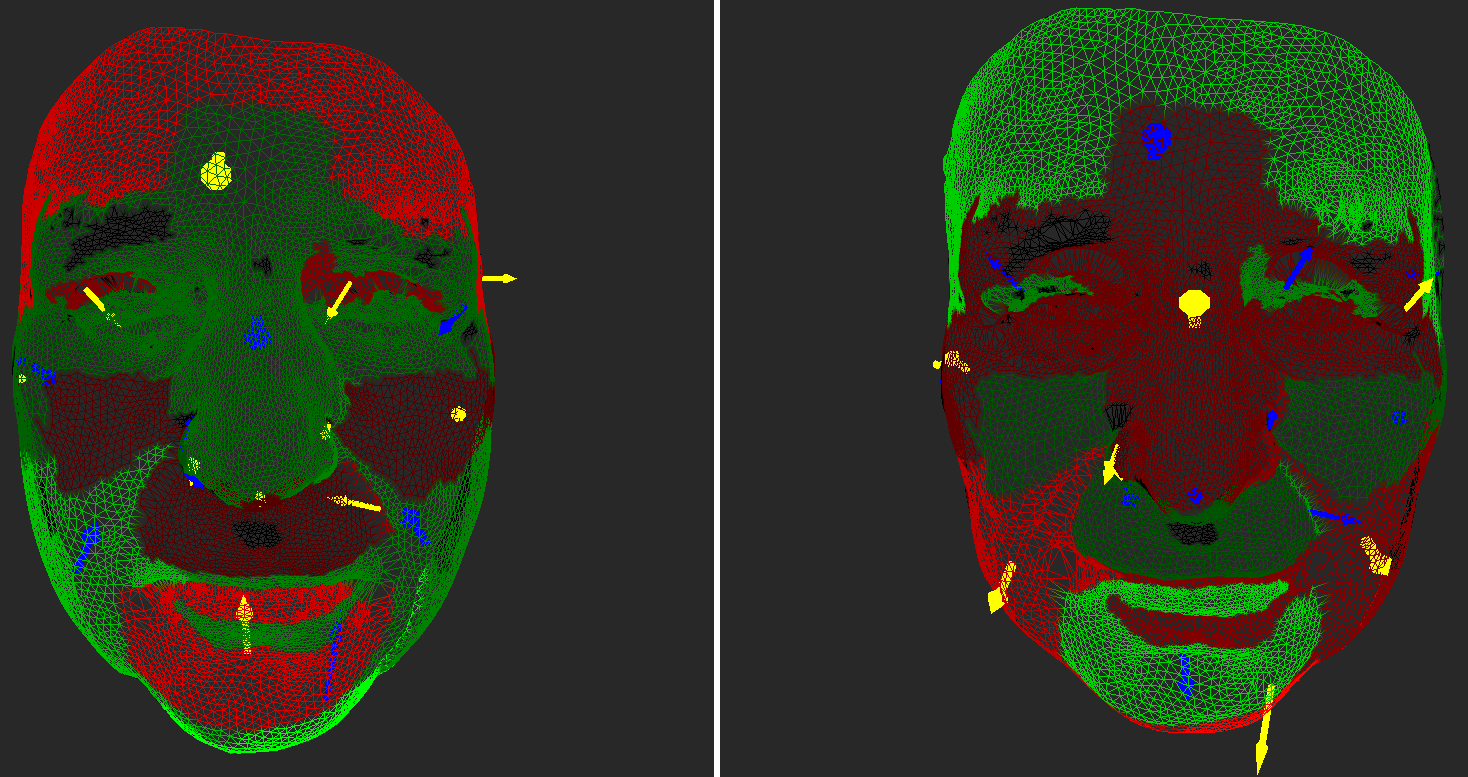
\includegraphics[width=\textwidth]{./screenshots/pair3.PNG}
\caption{}
\label{fig:0-3}
\end{subfigure}
\caption{Visualizations shown to the participants}
\end{figure}
\medskip

\begin{center}
\begin{tabular}{| c | c | c | c | c |}
	\hline
	Visualization & \ref{fig:0-2} & \ref{fig:0-4} & \ref{fig:0-1} & \ref{fig:0-3}\\ \hline
	\(\widehat{t}(p, q_1, V_k)\) & 20.46 & 26.19 & 20.26 & 21.56\\ \hline
	\multicolumn{5}{|c|}{\bf Answers} \\ \hline
	Left & 7 & 8 & 6 & 4\\ \hline
	Right & 4 & 2 & 1 & 2\\ \hline
	NotSure & 2 & 1 & 0 & 0\\ \hline
	{\bf Total} & {\bf 13} & {\bf 11} & {\bf 7} & {\bf 6}\\ \hline
\end{tabular}
\end{center}
\clearpage

\subsection{Question 2}
\label{sec:study-question2}

\begin{center}{\it Does the chin stick out more to the front in the right face than in the left face?}\end{center}

\begin{figure}[h]
\centering
\begin{subfigure}{0.4\textwidth}
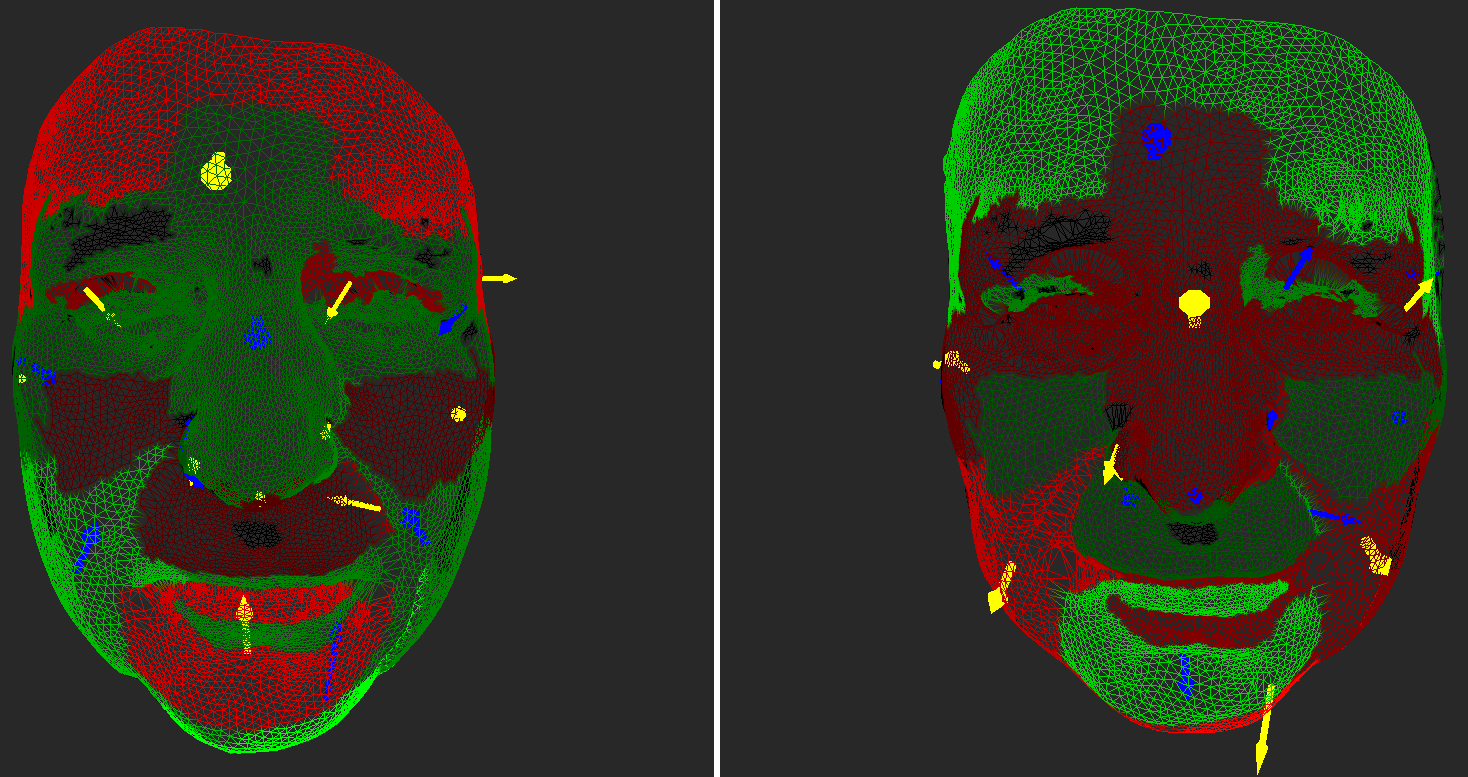
\includegraphics[width=\textwidth]{./screenshots/pair3.PNG}
\caption{}
\label{fig:1-3}
\end{subfigure}
\quad
\begin{subfigure}{0.4\textwidth}
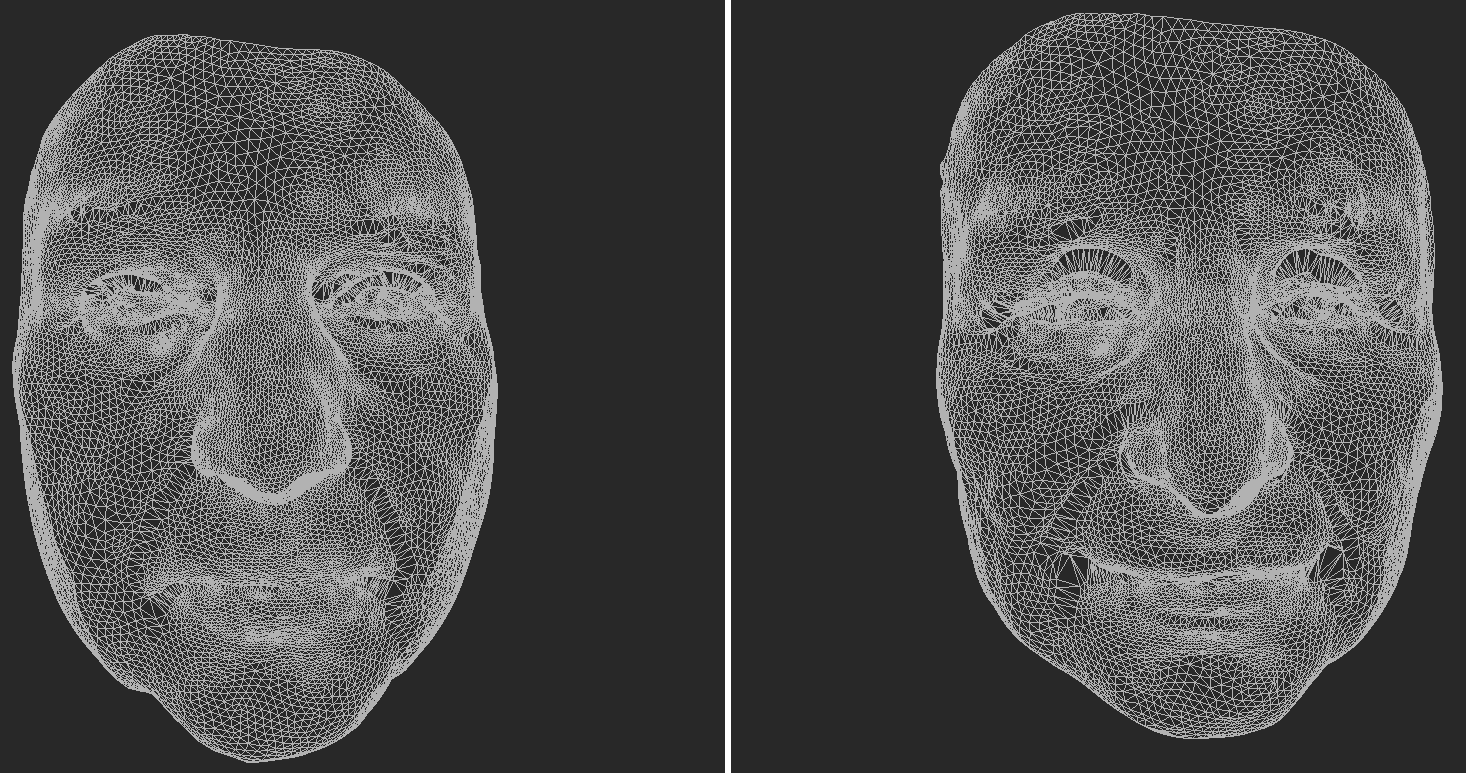
\includegraphics[width=\textwidth]{./screenshots/pair1.PNG}
\caption{}
\label{fig:1-1}
\end{subfigure}

\begin{subfigure}{0.4\textwidth}
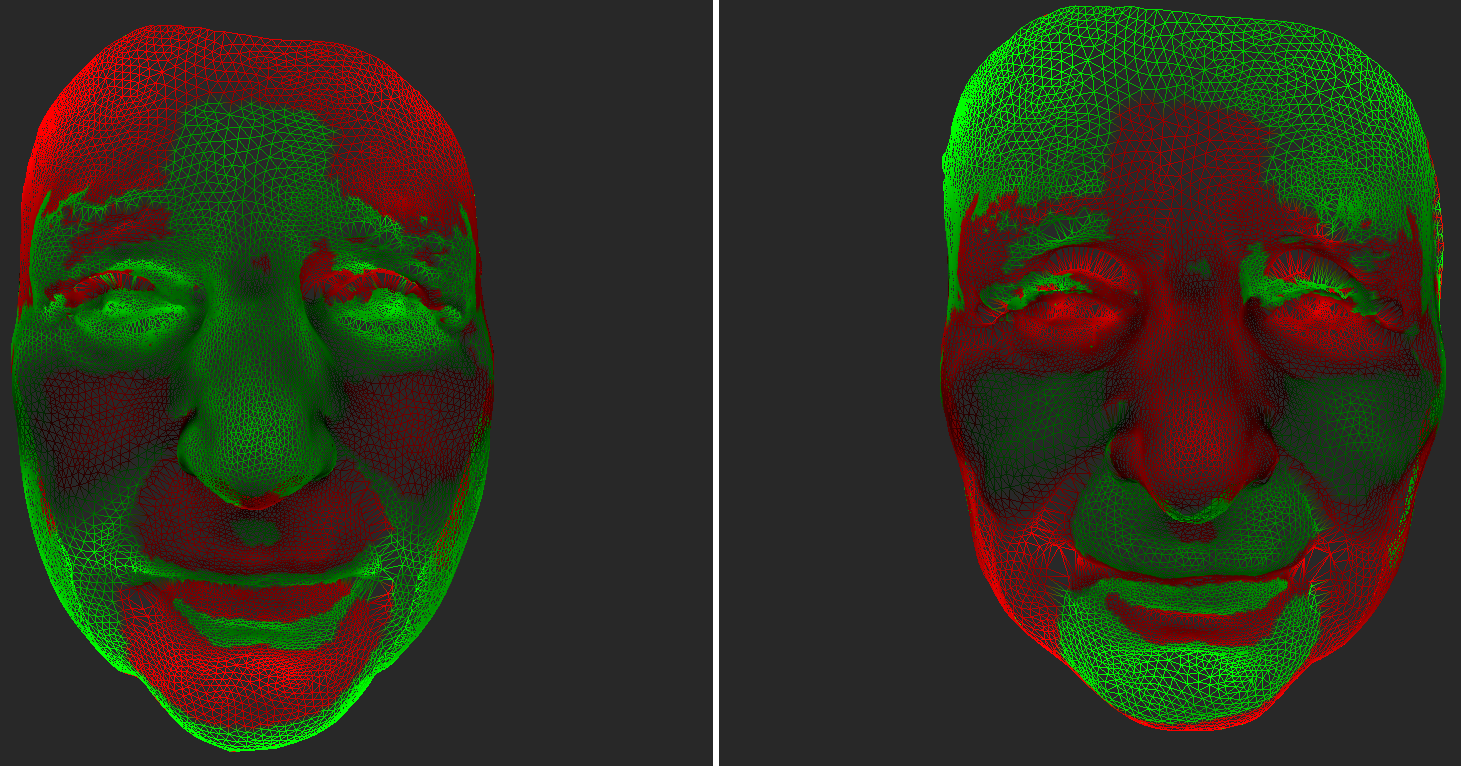
\includegraphics[width=\textwidth]{./screenshots/pair2.PNG}
\caption{}
\label{fig:1-2}
\end{subfigure}
\quad
\begin{subfigure}{0.4\textwidth}
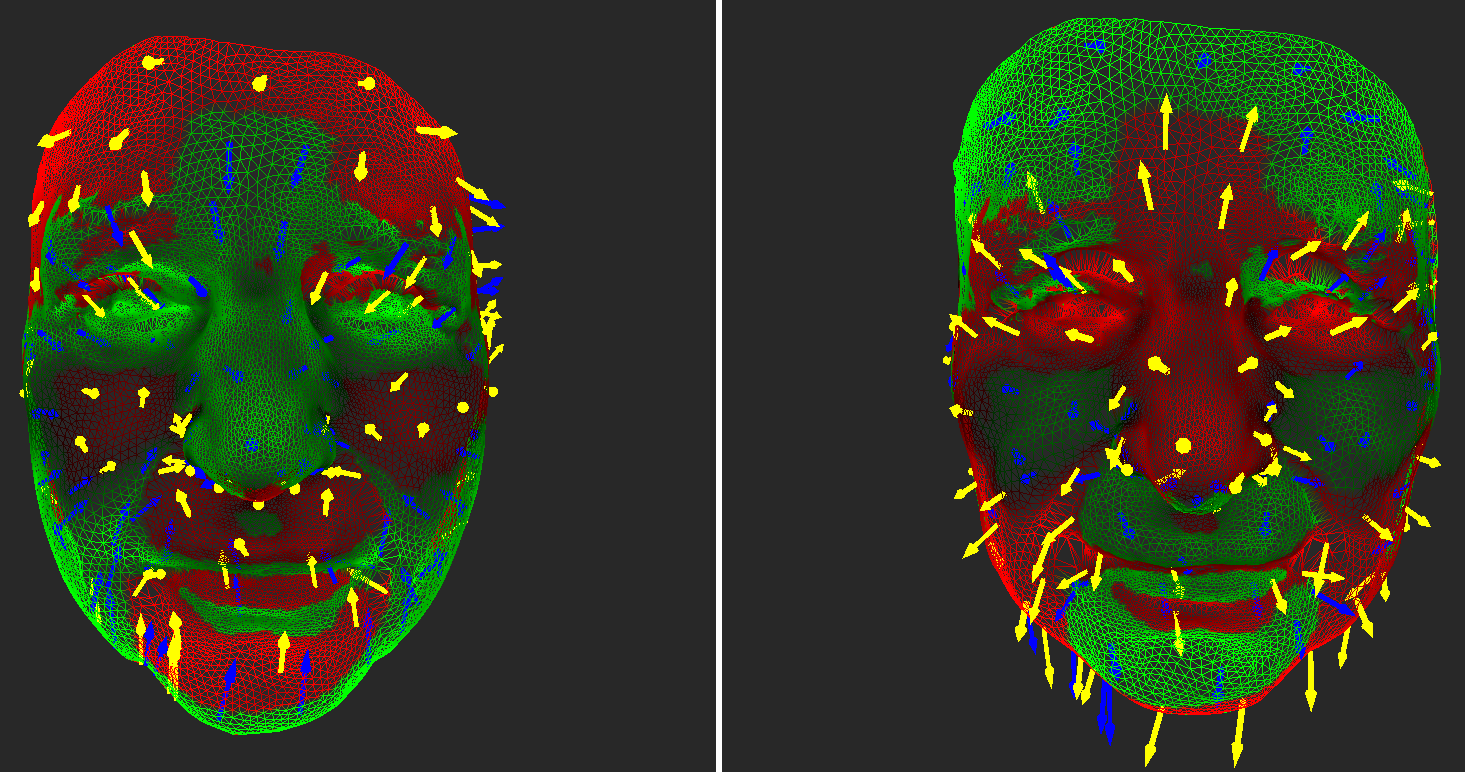
\includegraphics[width=\textwidth]{./screenshots/pair4.PNG}
\caption{}
\label{fig:1-4}
\end{subfigure}
\caption{Visualizations shown to the participants}
\end{figure}
\medskip

\begin{center}
\begin{tabular}{| c | c | c | c | c |}
	\hline
	Visualization & \ref{fig:1-3} & \ref{fig:1-1} & \ref{fig:1-2} & \ref{fig:1-4}\\ \hline
	\(\widehat{t}(p, q_2, V_k)\) & 46.62 & 43.08 & 61.56 & 38.90\\ \hline
	\multicolumn{5}{|c|}{\bf Answers} \\ \hline
	Yes & 10 & 5 & 6 & 4\\ \hline
	No & 3 & 4 & 1 & 2\\ \hline
	NotSure & 0 & 2 & 0 & 0\\ \hline
	{\bf Total} & {\bf 13} & {\bf 11} & {\bf 7} & {\bf 6}\\ \hline
\end{tabular}
\end{center}
\clearpage

\subsection{Question 3}
\label{sec:study-question3}

\begin{center}{\it Where is the most significant difference between the two faces?}\end{center}

\begin{figure}[h]
\centering
\begin{subfigure}{0.4\textwidth}
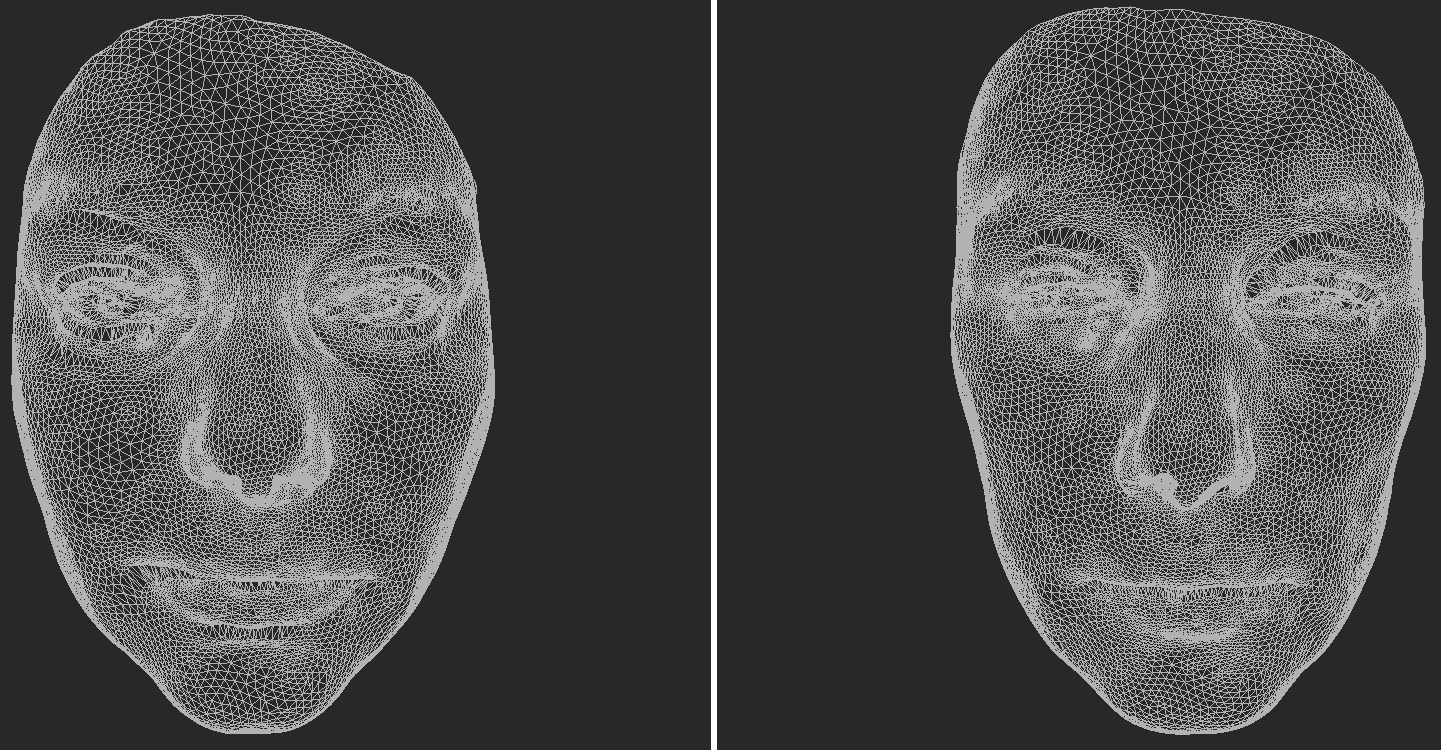
\includegraphics[width=\textwidth]{./screenshots/pair6.PNG}
\caption{}
\label{fig:2-6}
\end{subfigure}
\quad
\begin{subfigure}{0.4\textwidth}
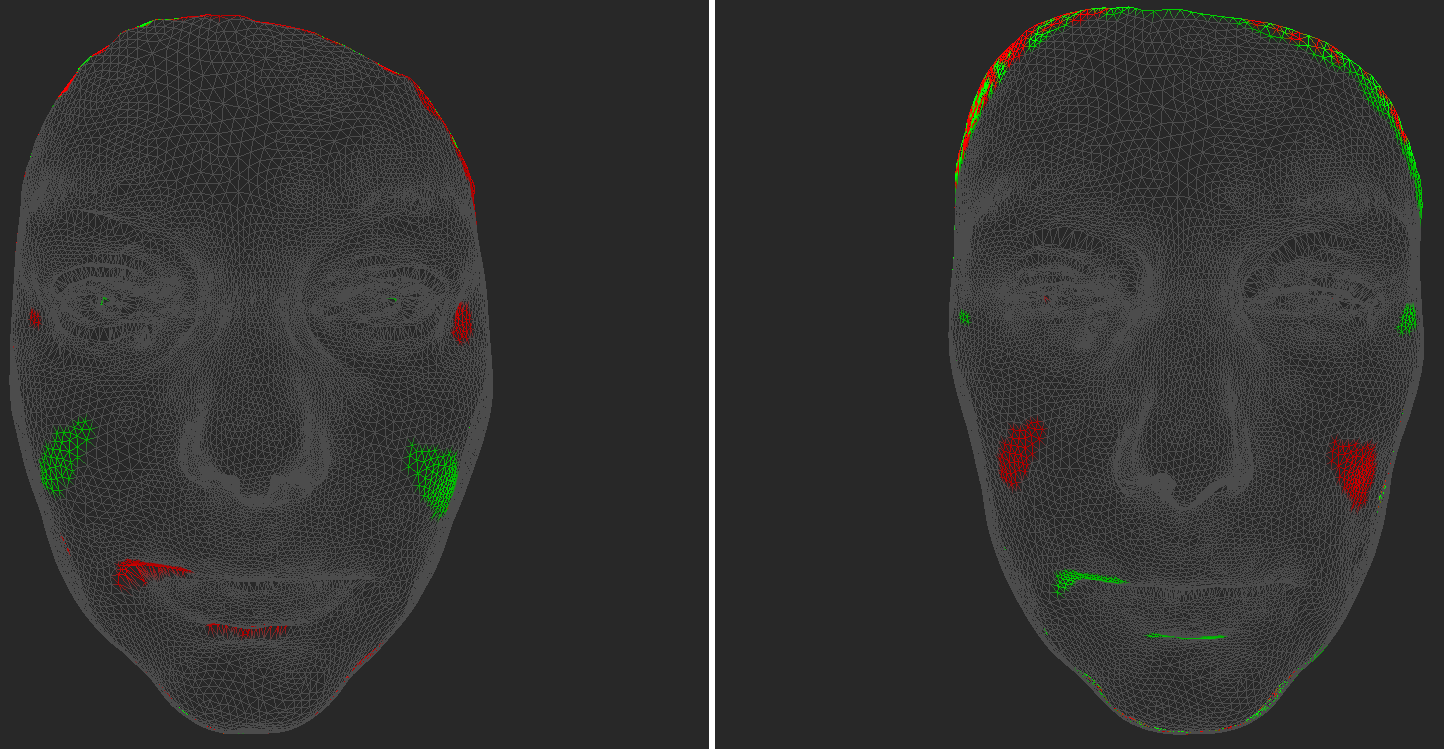
\includegraphics[width=\textwidth]{./screenshots/pair8.PNG}
\caption{}
\label{fig:2-8}
\end{subfigure}

\begin{subfigure}{0.4\textwidth}
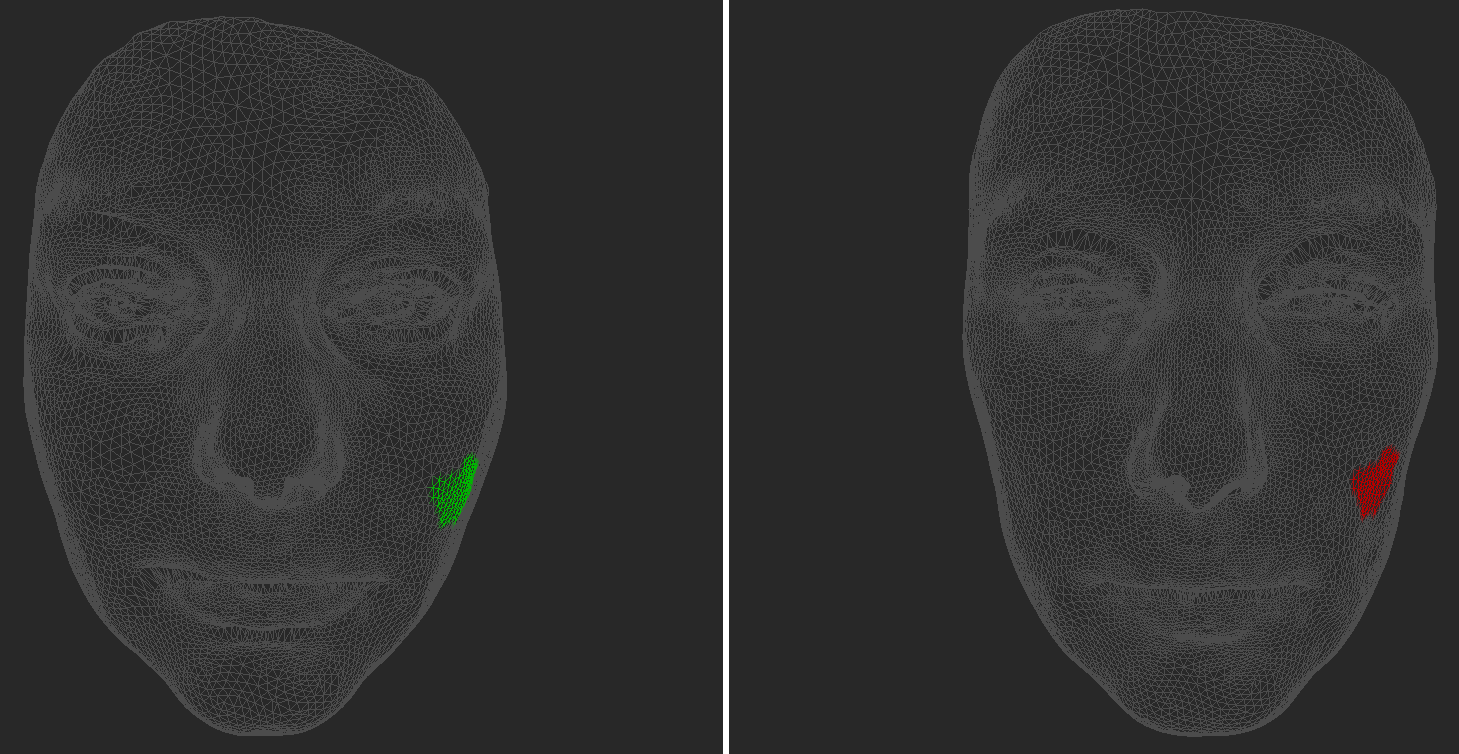
\includegraphics[width=\textwidth]{./screenshots/pair5.PNG}
\caption{}
\label{fig:2-5}
\end{subfigure}
\quad
\begin{subfigure}{0.4\textwidth}
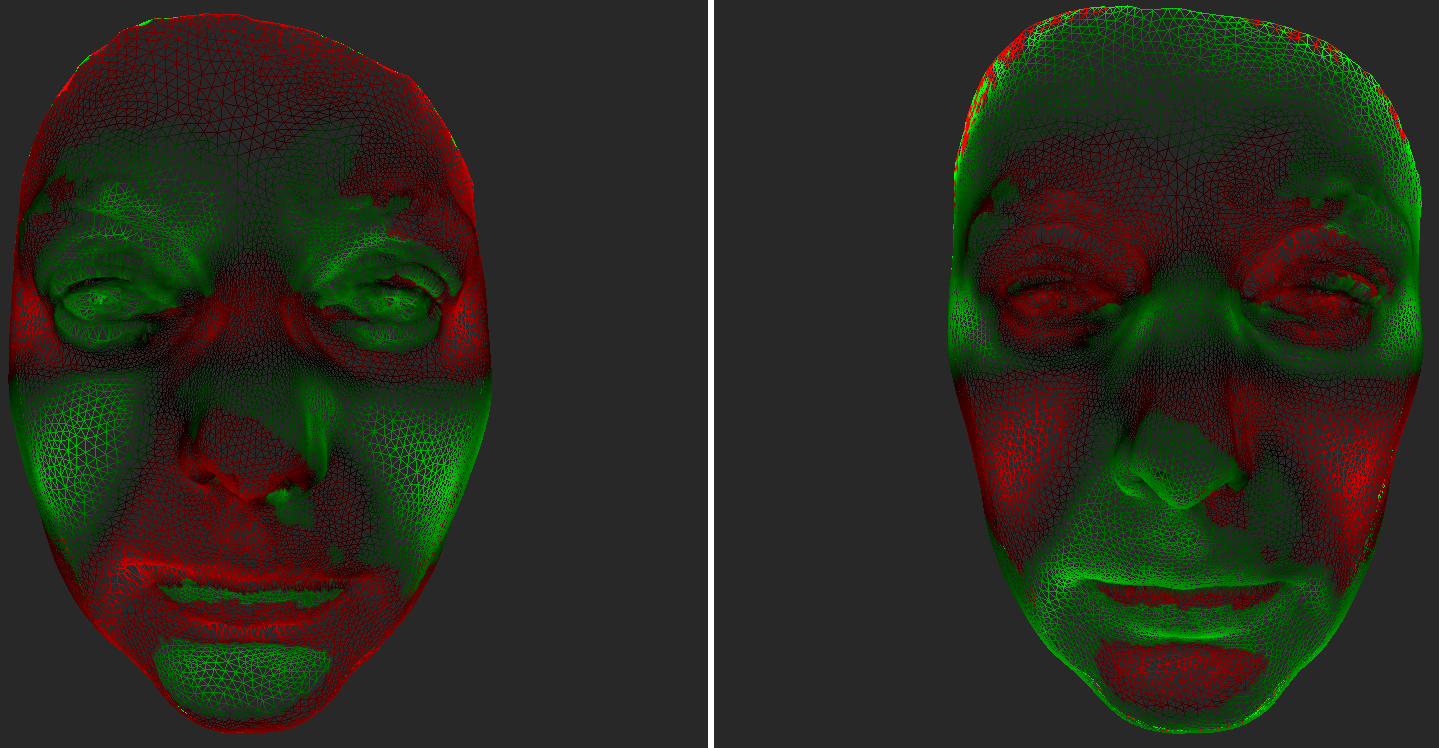
\includegraphics[width=\textwidth]{./screenshots/pair7.PNG}
\caption{}
\label{fig:2-7}
\end{subfigure}
\caption{Visualizations shown to the participants}
\end{figure}
\medskip

\begin{center}
\begin{tabular}{| c | c | c | c | c |}
	\hline
	Visualization & \ref{fig:2-6} & \ref{fig:2-8} & \ref{fig:2-5} & \ref{fig:2-7}\\ \hline
	\(\widehat{t}(p, q_3, V_k)\) & 41.87 & 37.36 & 31.29 & 58.84\\ \hline
	\multicolumn{5}{|c|}{\bf Answers} \\ \hline
	LeftCheek & 2 & 1 & 3 & 1\\ \hline
	Forehead & 5 & 4 & 0 & 1\\ \hline
	RightCheek & 2 & 4 & 2 & 1\\ \hline
	Nose & 1 & 0 & 0 & 0\\ \hline
	NotSure & 2 & 2 & 1 & 1\\ \hline
	Chin & 1 & 0 & 0 & 0\\ \hline
	Mouth & 0 & 0 & 1 & 2\\ \hline
	{\bf Total} & {\bf 13} & {\bf 11} & {\bf 7} & {\bf 6}\\ \hline
\end{tabular}
\end{center}
\clearpage

\subsection{Question 4}
\label{sec:study-question4}

\begin{center}{\it When examining the differences moving from the left face to the right face, what is their main direction in the area below the nose?}\end{center}

\begin{figure}[h]
\centering
\begin{subfigure}{0.4\textwidth}
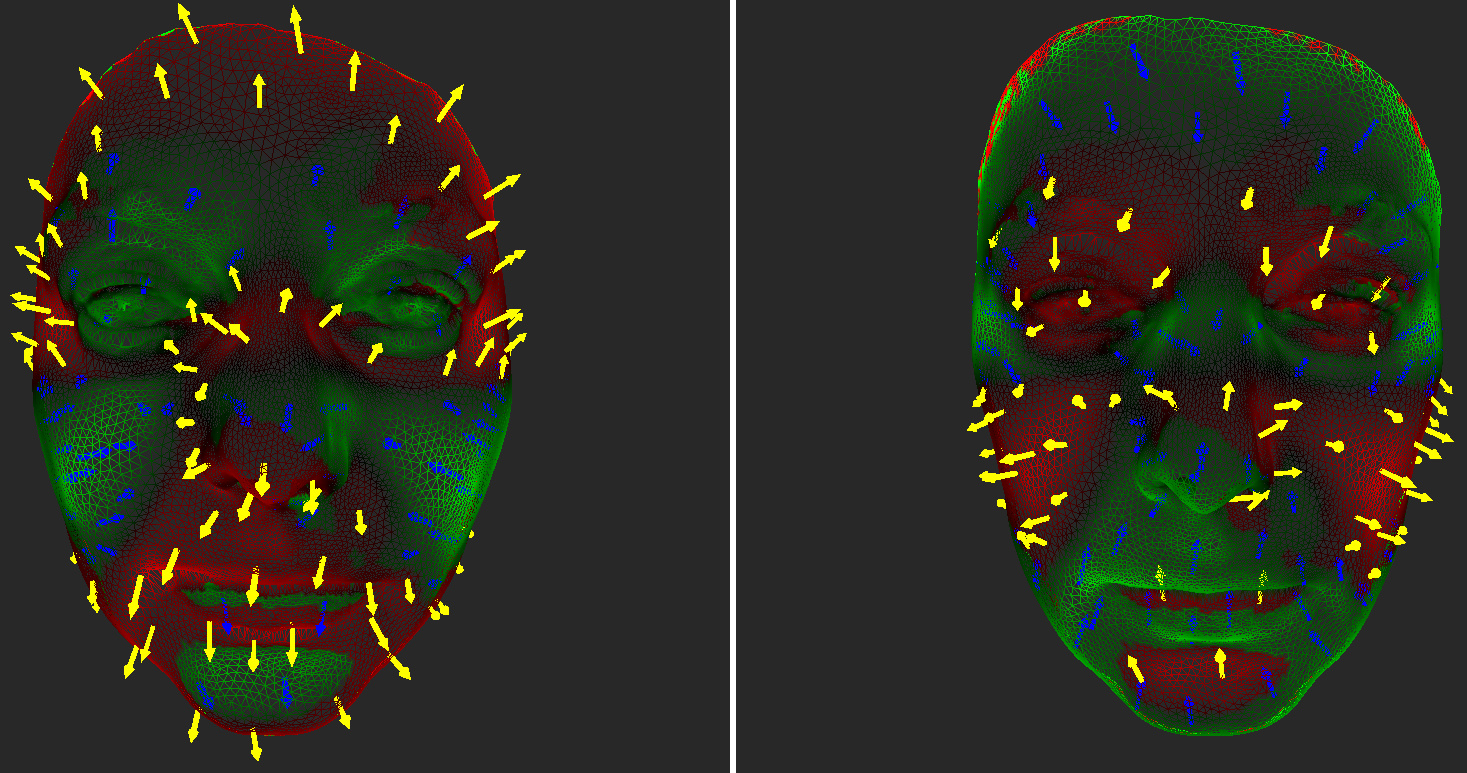
\includegraphics[width=\textwidth]{./screenshots/pair10.PNG}
\caption{}
\label{fig:3-10}
\end{subfigure}
\quad
\begin{subfigure}{0.4\textwidth}
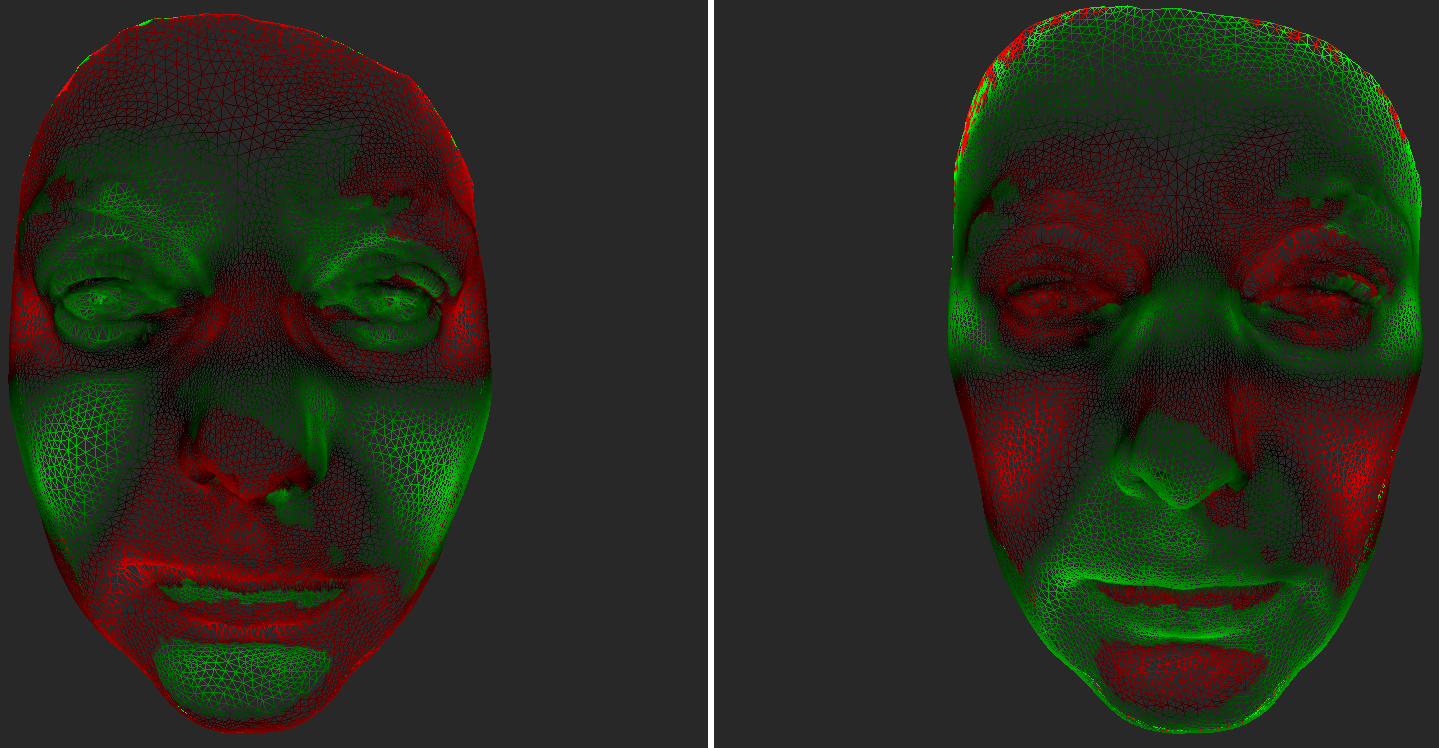
\includegraphics[width=\textwidth]{./screenshots/pair7.PNG}
\caption{}
\label{fig:3-7}
\end{subfigure}

\begin{subfigure}{0.4\textwidth}
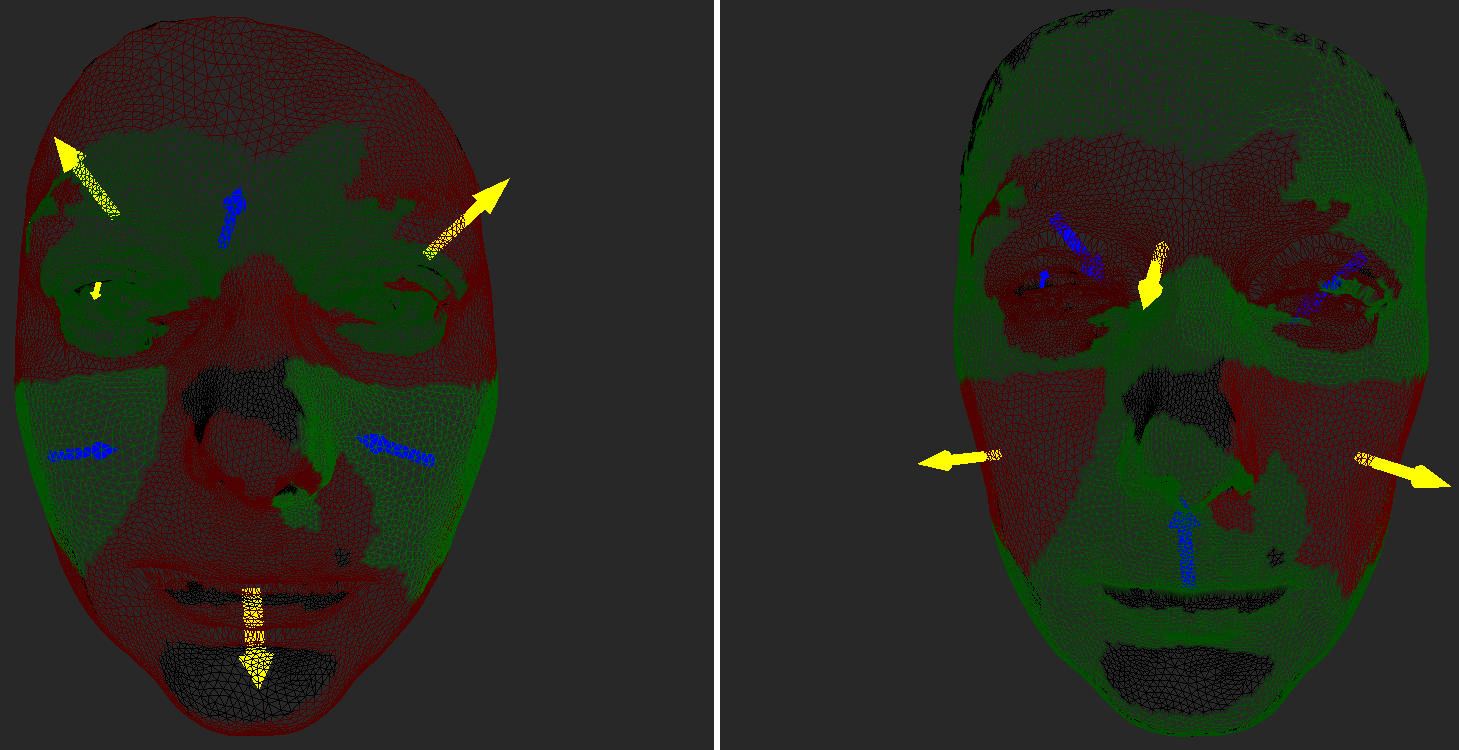
\includegraphics[width=\textwidth]{./screenshots/pair9.PNG}
\caption{}
\label{fig:3-9}
\end{subfigure}
\quad
\begin{subfigure}{0.4\textwidth}
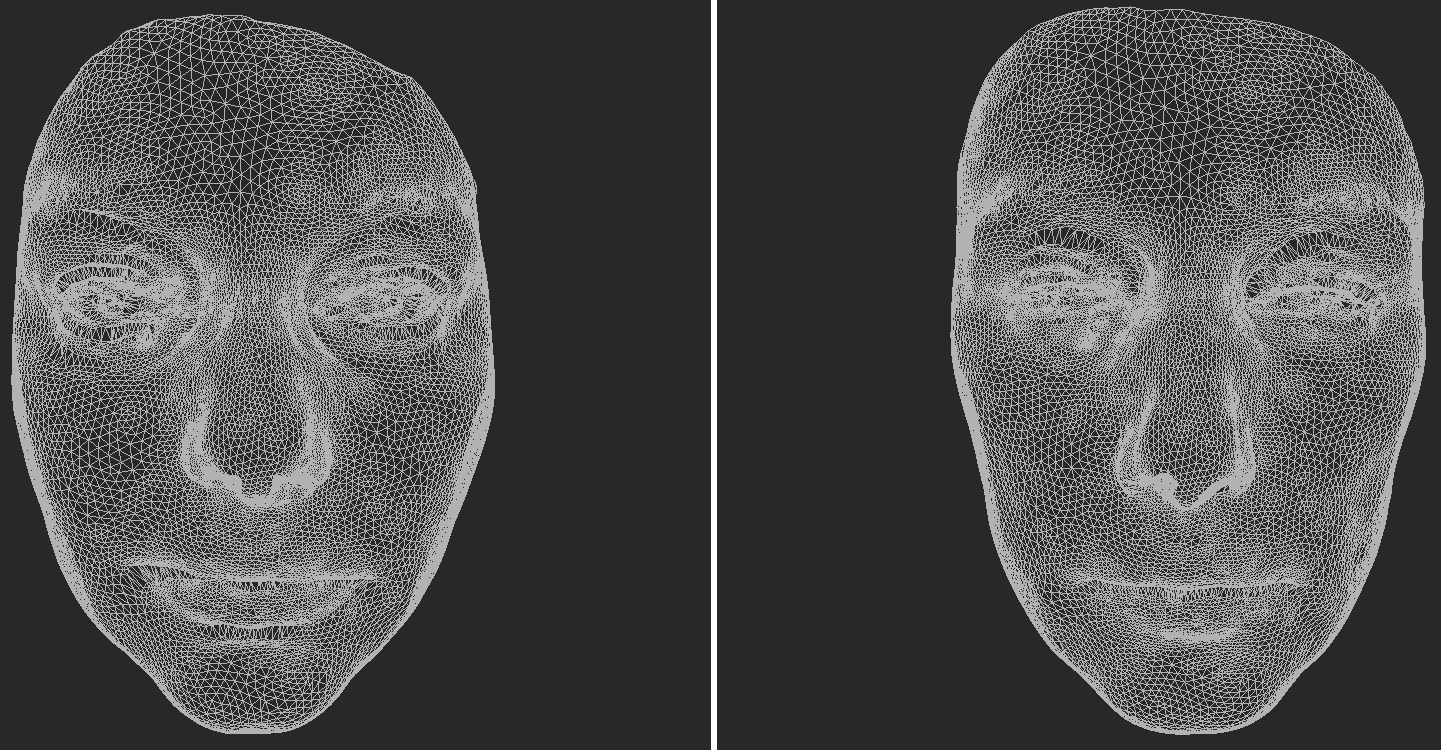
\includegraphics[width=\textwidth]{./screenshots/pair6.PNG}
\caption{}
\label{fig:3-6}
\end{subfigure}
\caption{Visualizations shown to the participants}
\end{figure}
\medskip

\begin{center}
\begin{tabular}{| c | c | c | c | c |}
	\hline
	Visualization & \ref{fig:3-10} & \ref{fig:3-7} & \ref{fig:3-9} & \ref{fig:3-6}\\ \hline
	\(\widehat{t}(p, q_4, V_k)\) & 48.19 & 53.41 & 47.80 & 55.13\\ \hline
	\multicolumn{5}{|c|}{\bf Answers} \\ \hline
	Down & 5 & 2 & 2 & 1\\ \hline
	Right & 1 & 0 & 0 & 1\\ \hline
	In & 2 & 2 & 1 & 0\\ \hline
	NotSure & 2 & 1 & 2 & 2\\ \hline
	Left & 1 & 1 & 0 & 0\\ \hline
	Out & 2 & 5 & 0 & 1\\ \hline
	Up & 0 & 0 & 2 & 1\\ \hline
	{\bf Total} & {\bf 13} & {\bf 11} & {\bf 7} & {\bf 6}\\ \hline
\end{tabular}
\end{center}
\clearpage

\subsection{Question 5}
\label{sec:study-question5}

\begin{center}{\it Does the left cheek stick out more to the front in the right face than in the left face?}\end{center}

\begin{figure}[h]
\centering
\begin{subfigure}{0.4\textwidth}
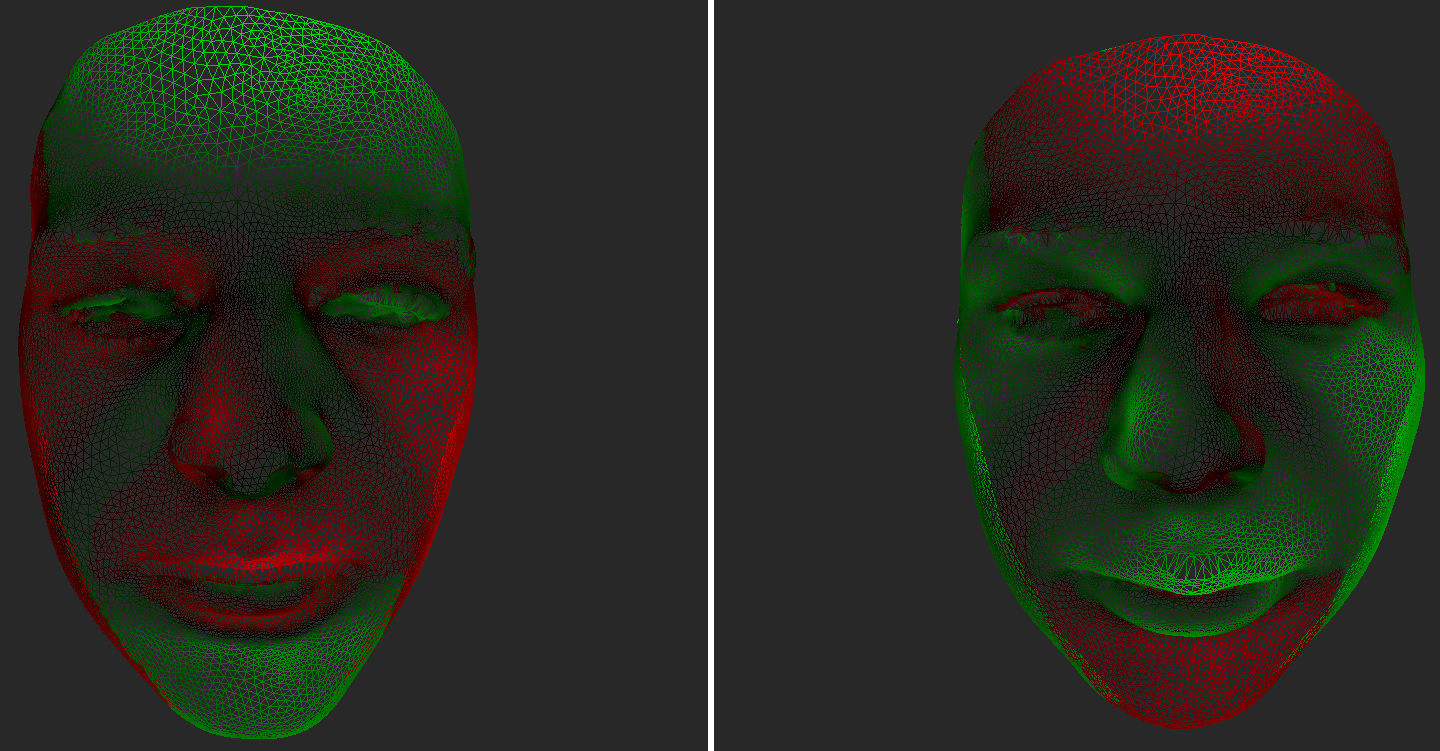
\includegraphics[width=\textwidth]{./screenshots/pair12.PNG}
\caption{}
\label{fig:4-12}
\end{subfigure}
\quad
\begin{subfigure}{0.4\textwidth}
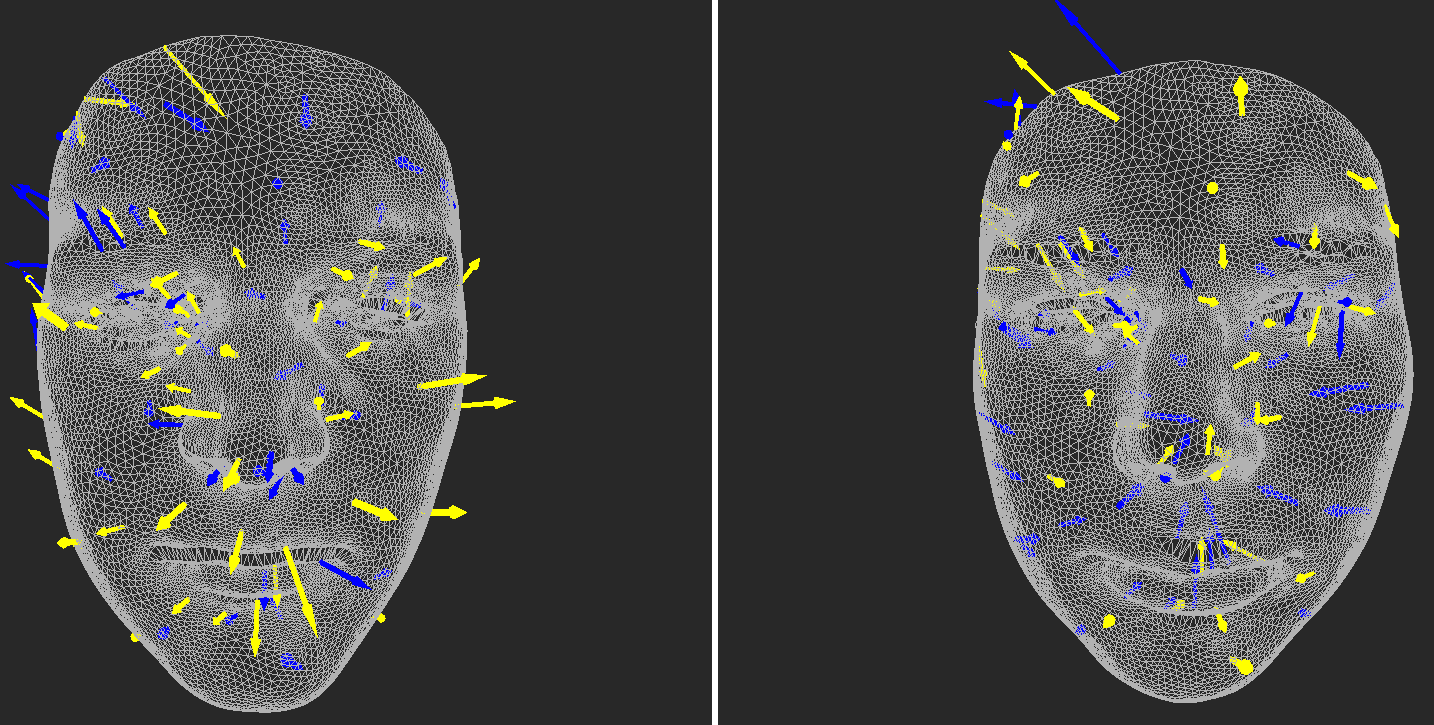
\includegraphics[width=\textwidth]{./screenshots/pair14.PNG}
\caption{}
\label{fig:4-14}
\end{subfigure}

\begin{subfigure}{0.4\textwidth}
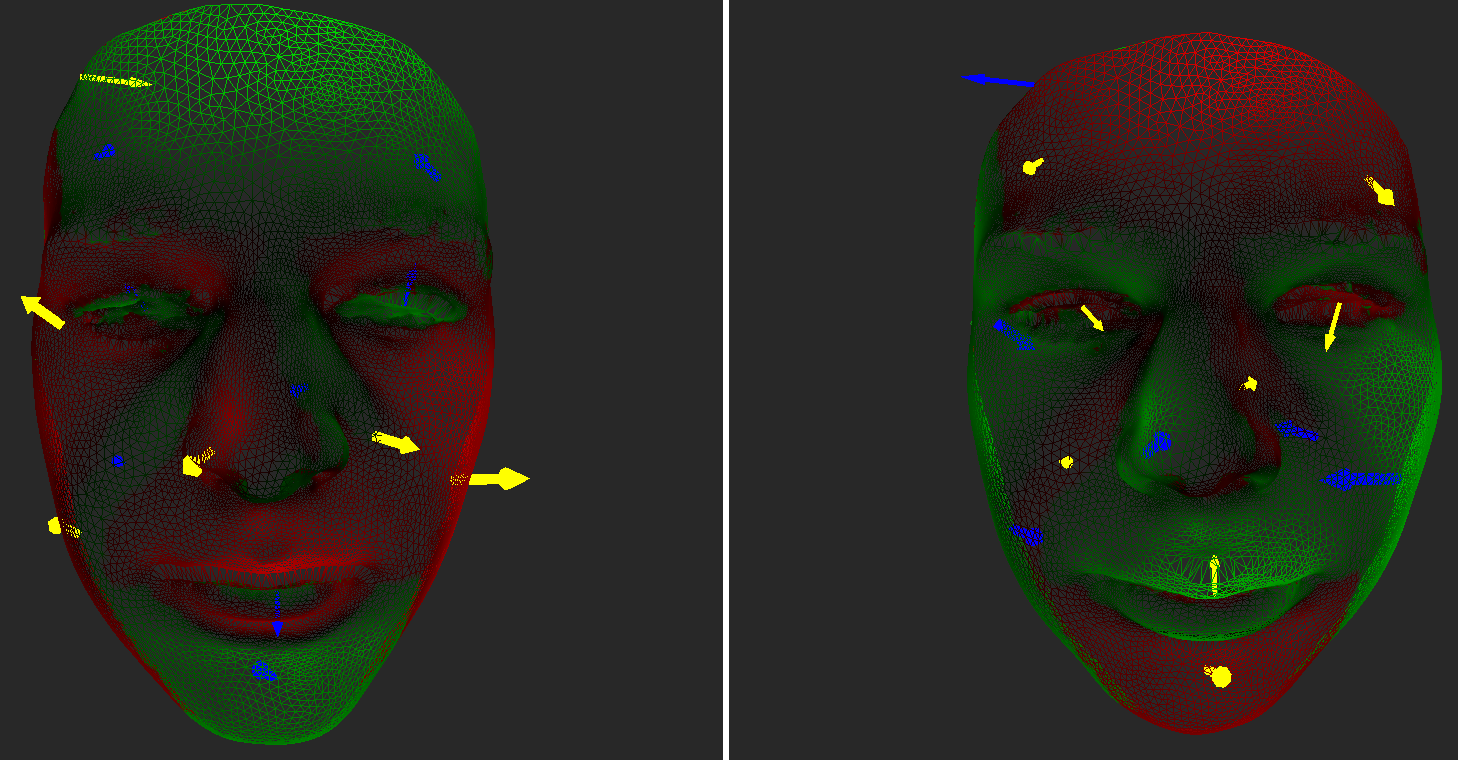
\includegraphics[width=\textwidth]{./screenshots/pair11.PNG}
\caption{}
\label{fig:4-11}
\end{subfigure}
\quad
\begin{subfigure}{0.4\textwidth}
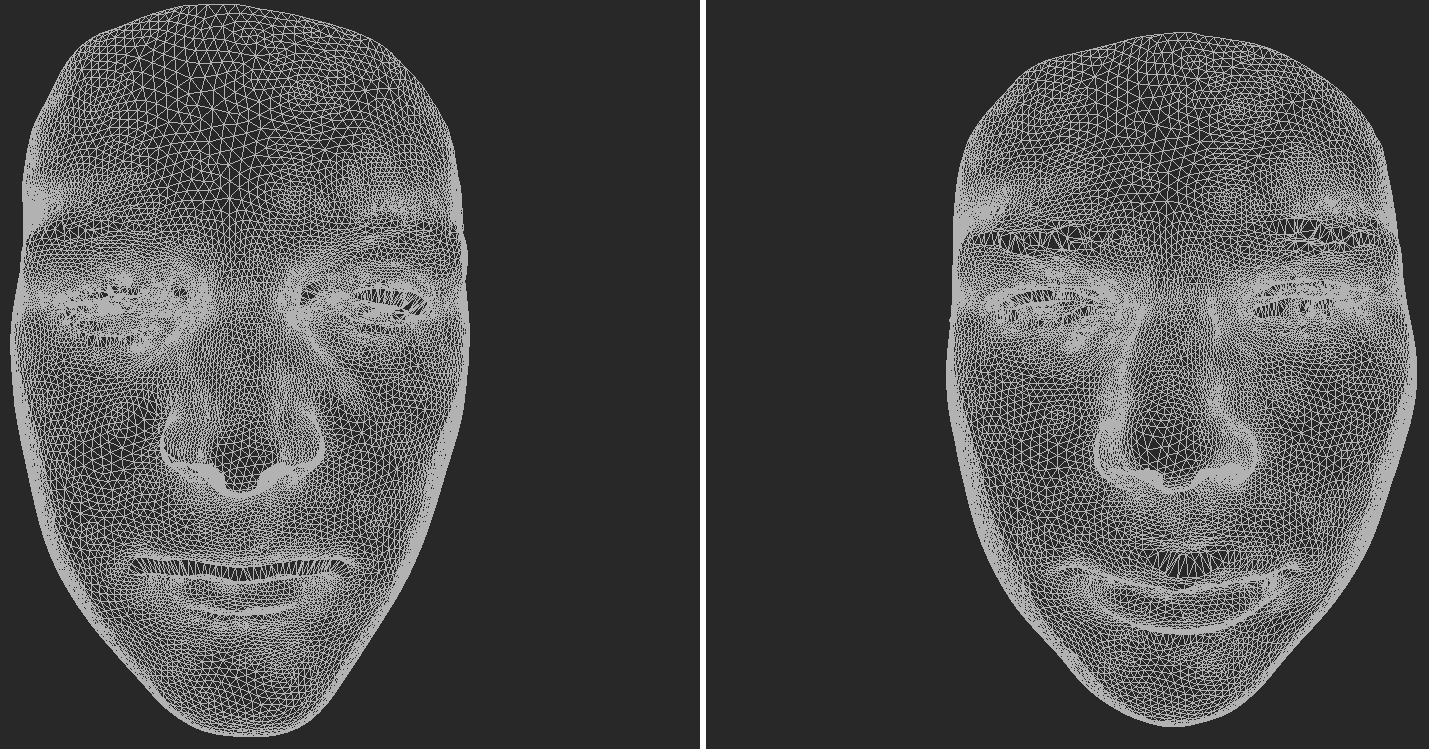
\includegraphics[width=\textwidth]{./screenshots/pair13.PNG}
\caption{}
\label{fig:4-13}
\end{subfigure}
\caption{Visualizations shown to the participants}
\end{figure}
\medskip

\begin{center}
\begin{tabular}{| c | c | c | c | c |}
	\hline
	Visualization & \ref{fig:4-12} & \ref{fig:4-14} & \ref{fig:4-11} & \ref{fig:4-13}\\ \hline
	\(\widehat{t}(p, q_5, V_k)\) & 40.74 & 43.85 & 49.87 & 31.33\\ \hline
	\multicolumn{5}{|c|}{\bf Answers} \\ \hline
	Yes & 8 & 5 & 6 & 3\\ \hline
	No & 5 & 6 & 1 & 3\\ \hline
	{\bf Total} & {\bf 13} & {\bf 11} & {\bf 7} & {\bf 6}\\ \hline
\end{tabular}
\end{center}
\clearpage

\subsection{Question 6}
\label{sec:study-question6}

\begin{center}{\it Which face has a longer nose?}\end{center}

\begin{figure}[h]
\centering
\begin{subfigure}{0.4\textwidth}
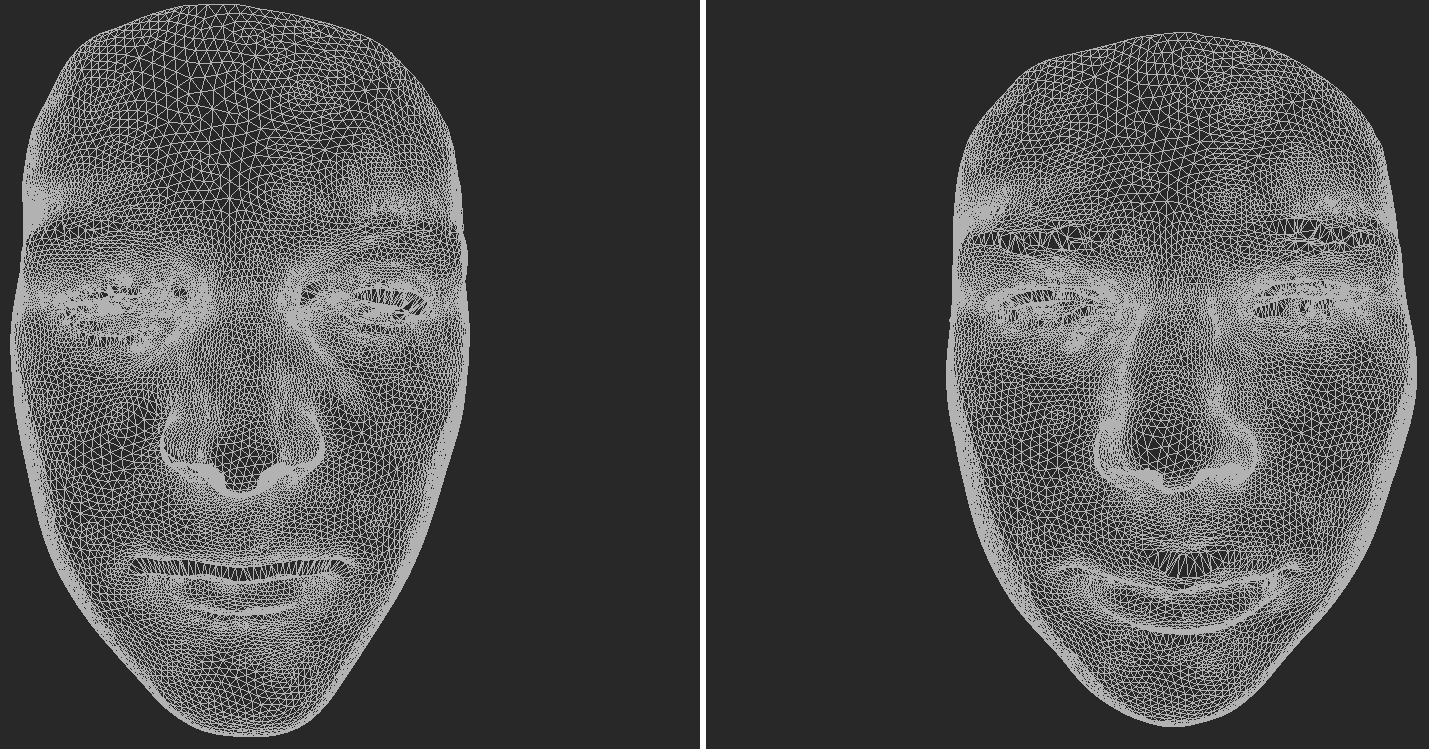
\includegraphics[width=\textwidth]{./screenshots/pair13.PNG}
\caption{}
\label{fig:5-13}
\end{subfigure}
\quad
\begin{subfigure}{0.4\textwidth}
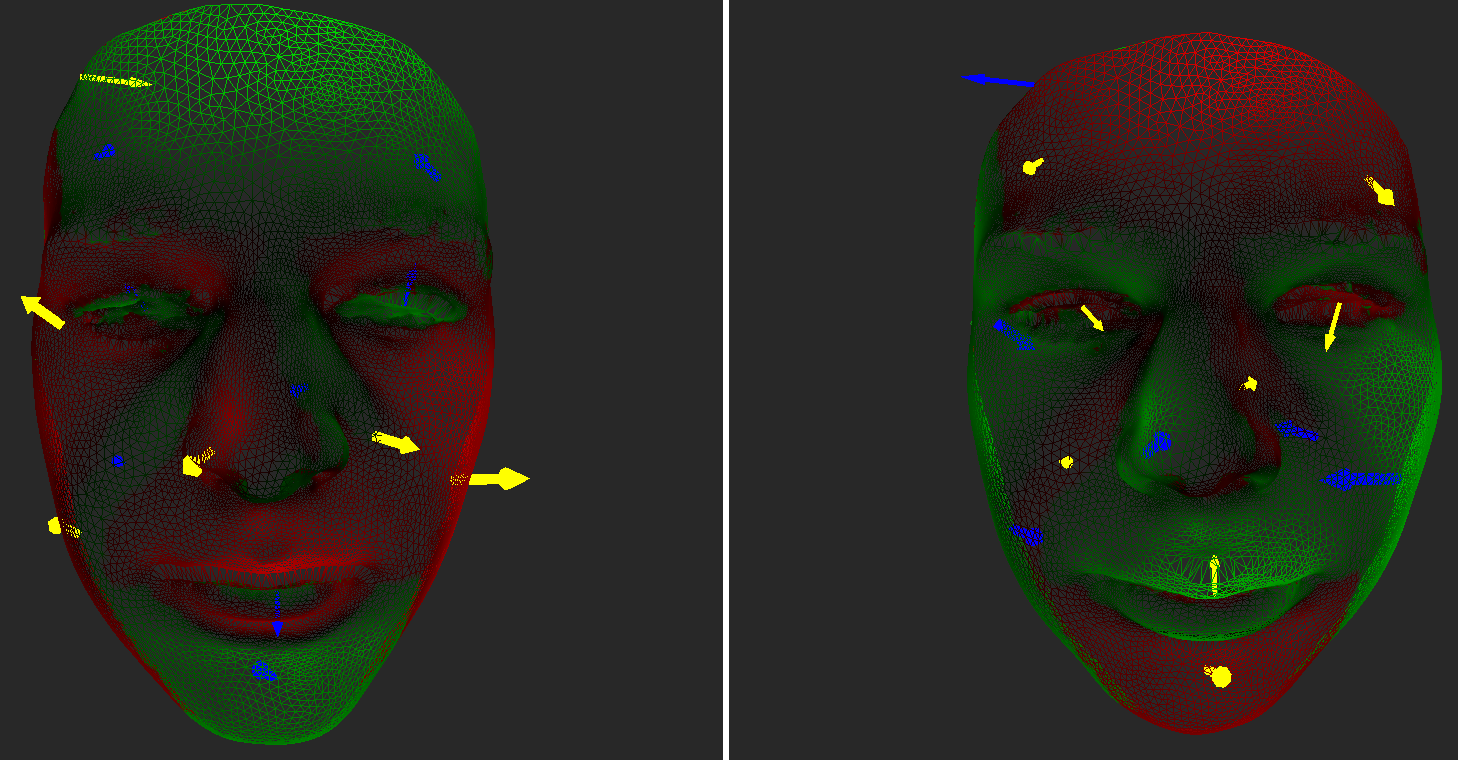
\includegraphics[width=\textwidth]{./screenshots/pair11.PNG}
\caption{}
\label{fig:5-11}
\end{subfigure}

\begin{subfigure}{0.4\textwidth}
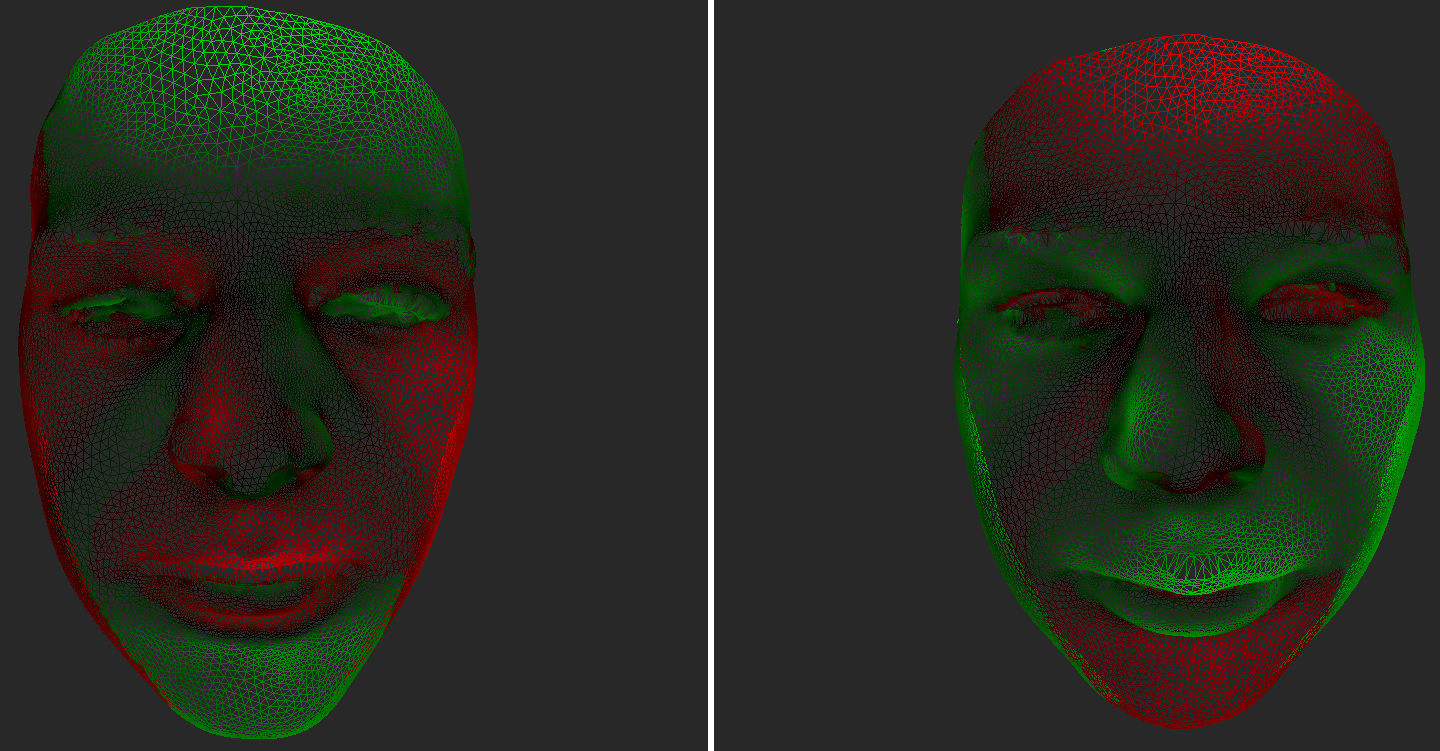
\includegraphics[width=\textwidth]{./screenshots/pair12.PNG}
\caption{}
\label{fig:5-12}
\end{subfigure}
\quad
\begin{subfigure}{0.4\textwidth}
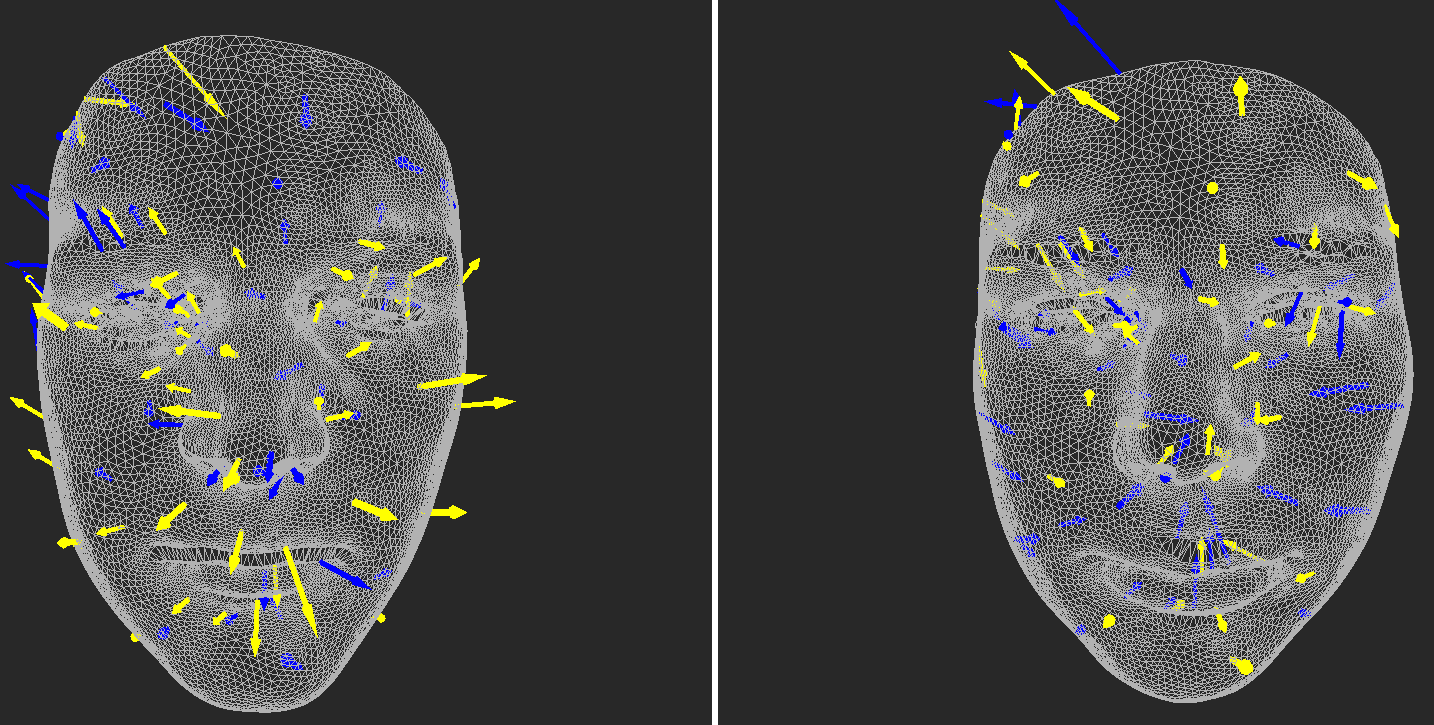
\includegraphics[width=\textwidth]{./screenshots/pair14.PNG}
\caption{}
\label{fig:5-14}
\end{subfigure}
\caption{Visualizations shown to the participants}
\end{figure}
\medskip

\begin{center}
\begin{tabular}{| c | c | c | c | c |}
	\hline
	Visualization & \ref{fig:5-13} & \ref{fig:5-11} & \ref{fig:5-12} & \ref{fig:5-14}\\ \hline
	\(\widehat{t}(p, q_6, V_k)\) & 33.37 & 32.34 & 23.85 & 29.71\\ \hline
	\multicolumn{5}{|c|}{\bf Answers} \\ \hline
	NotSure & 2 & 1 & 0 & 0\\ \hline
	Right & 3 & 5 & 3 & 1\\ \hline
	Left & 8 & 5 & 4 & 5\\ \hline
	{\bf Total} & {\bf 13} & {\bf 11} & {\bf 7} & {\bf 6}\\ \hline
\end{tabular}
\end{center}
\clearpage

\subsection{Question 7}
\label{sec:study-question7}

\begin{center}{\it Which face has larger cheekbones?}\end{center}

\begin{figure}[h]
\centering
\begin{subfigure}{0.4\textwidth}
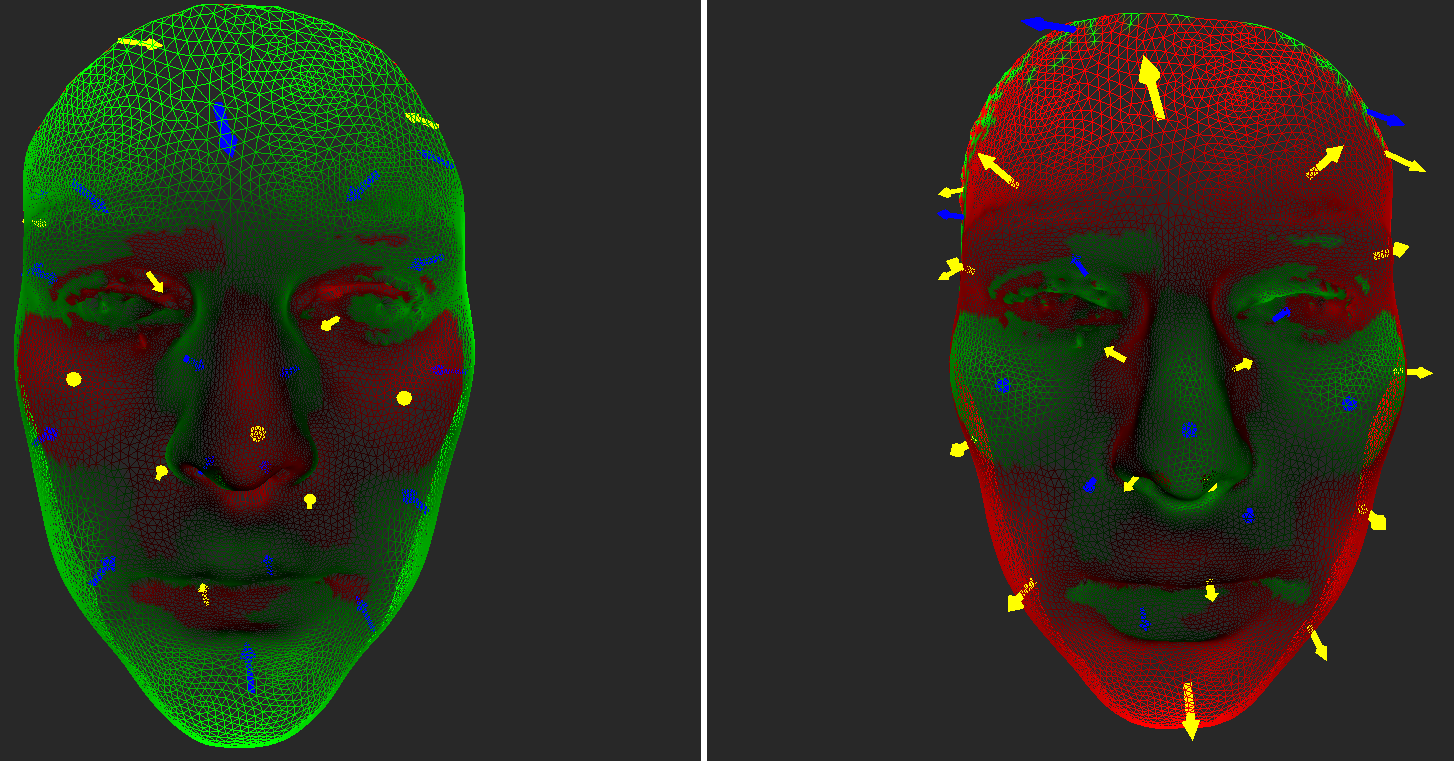
\includegraphics[width=\textwidth]{./screenshots/pair17.PNG}
\caption{}
\label{fig:6-17}
\end{subfigure}
\quad
\begin{subfigure}{0.4\textwidth}
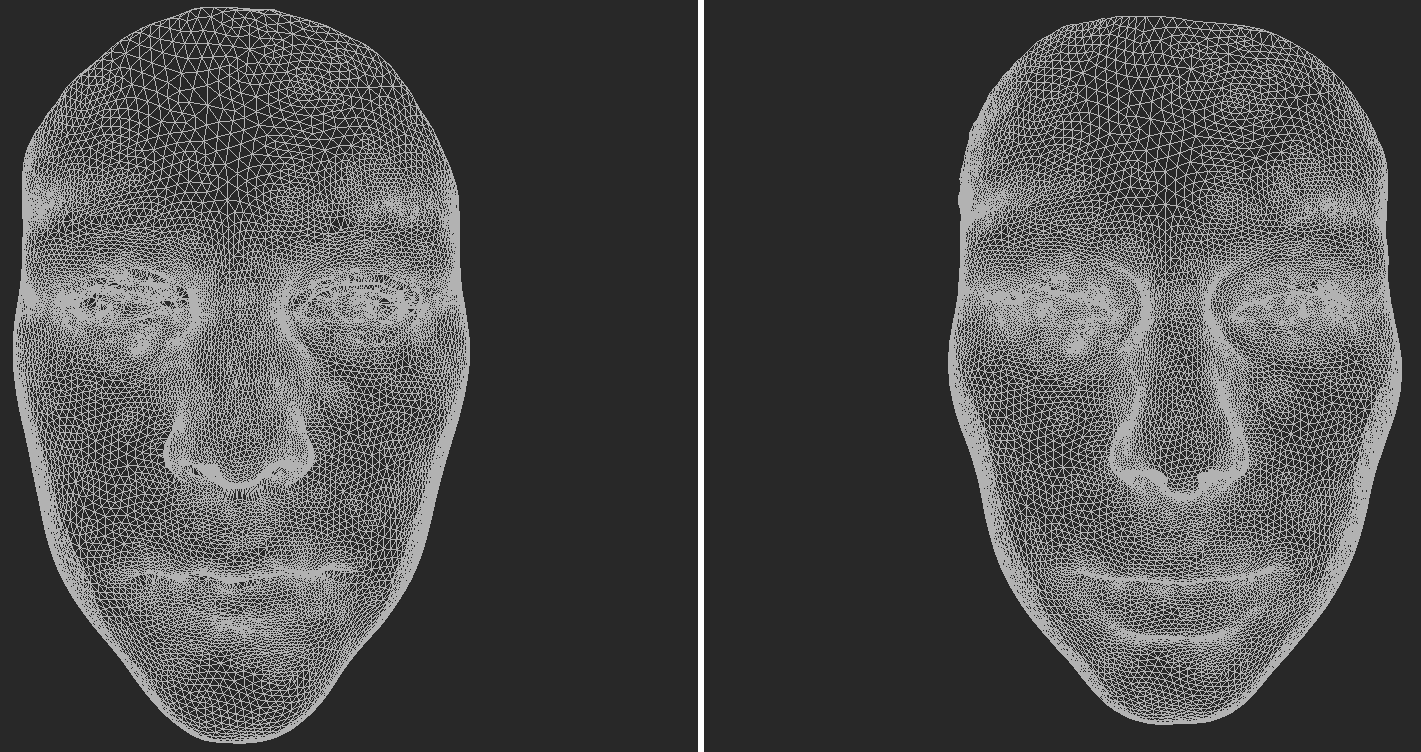
\includegraphics[width=\textwidth]{./screenshots/pair15.PNG}
\caption{}
\label{fig:6-15}
\end{subfigure}

\begin{subfigure}{0.4\textwidth}
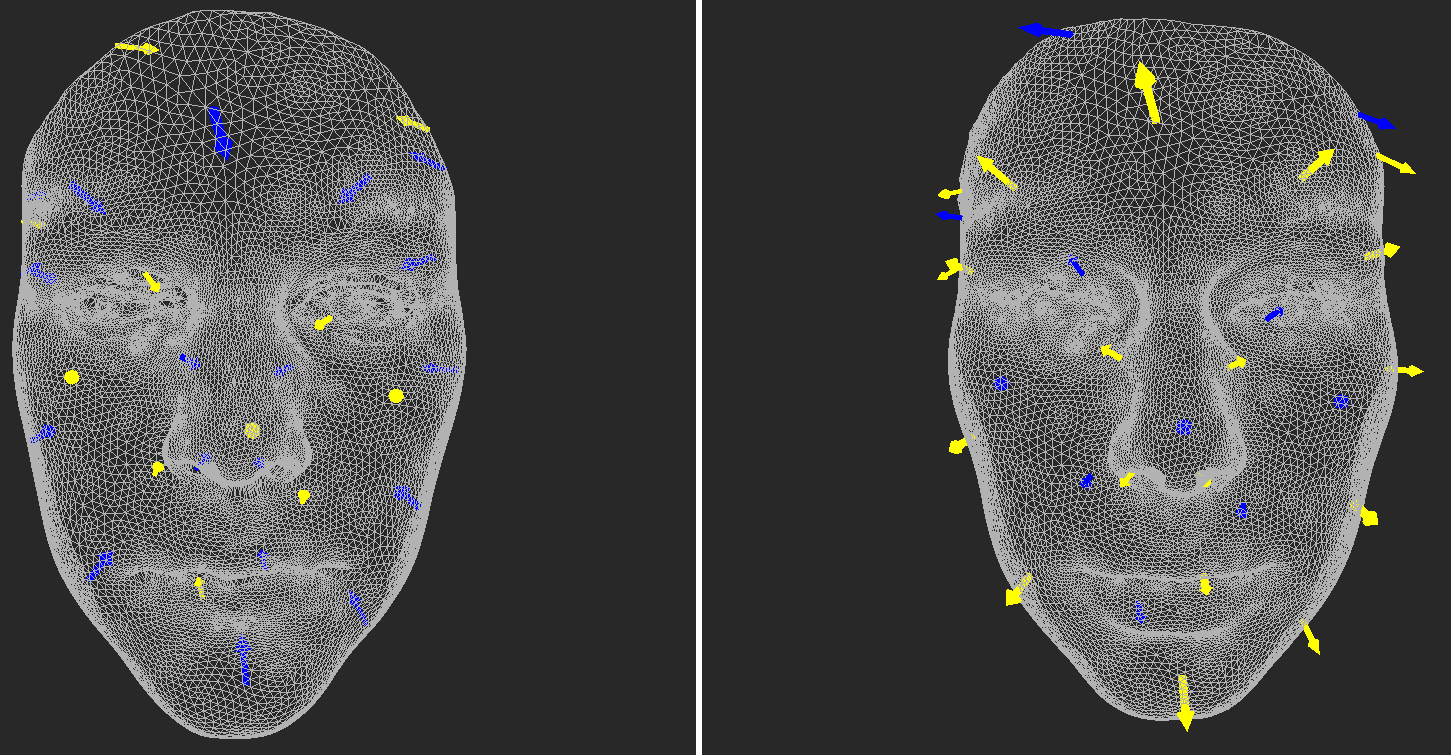
\includegraphics[width=\textwidth]{./screenshots/pair18.PNG}
\caption{}
\label{fig:6-18}
\end{subfigure}
\quad
\begin{subfigure}{0.4\textwidth}
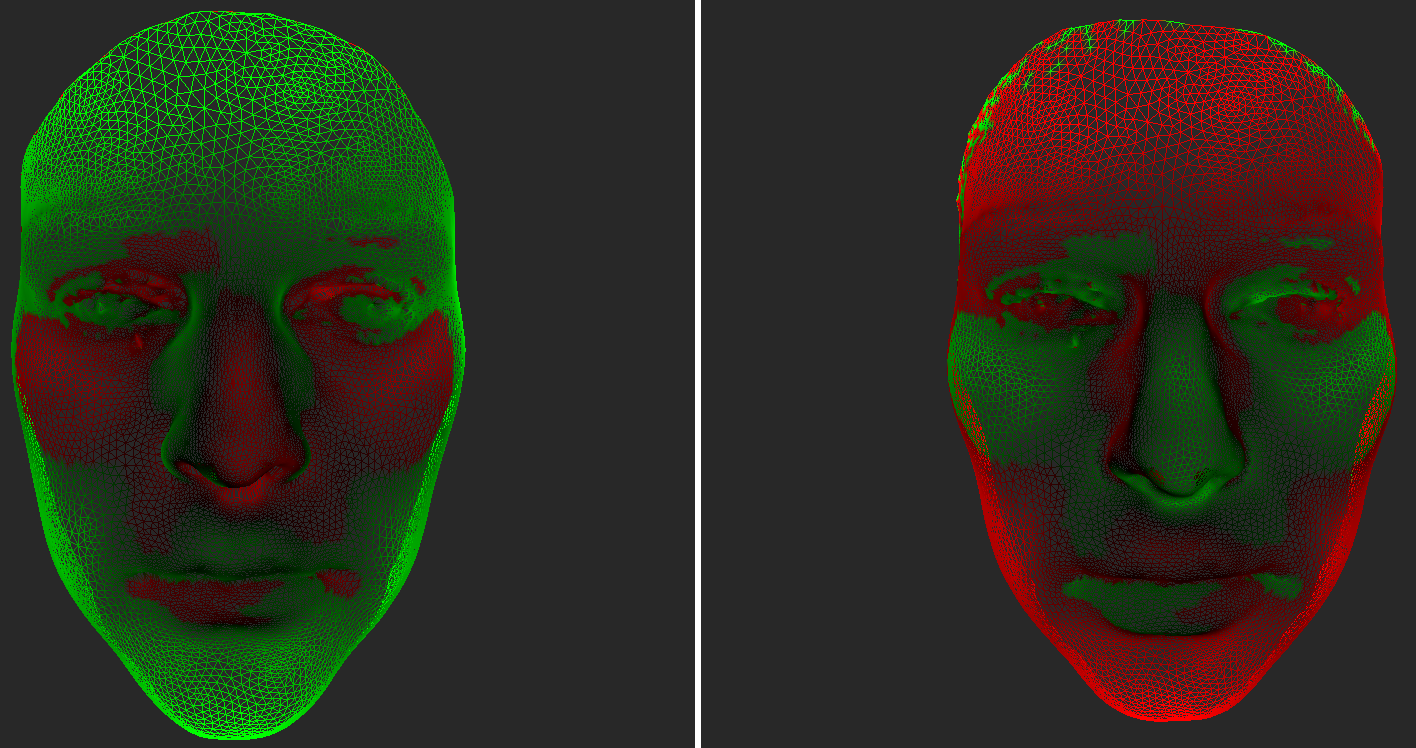
\includegraphics[width=\textwidth]{./screenshots/pair16.PNG}
\caption{}
\label{fig:6-16}
\end{subfigure}
\caption{Visualizations shown to the participants}
\end{figure}
\medskip

\begin{center}
\begin{tabular}{| c | c | c | c | c |}
	\hline
	Visualization & \ref{fig:6-17} & \ref{fig:6-15} & \ref{fig:6-18} & \ref{fig:6-16}\\ \hline
	\(\widehat{t}(p, q_7, V_k)\) & 16.11 & 24.59 & 18.47 & 15.01\\ \hline
	\multicolumn{5}{|c|}{\bf Answers} \\ \hline
	Right & 11 & 4 & 6 & 5\\ \hline
	Left & 2 & 4 & 0 & 1\\ \hline
	NotSure & 0 & 3 & 1 & 0\\ \hline
	{\bf Total} & {\bf 13} & {\bf 11} & {\bf 7} & {\bf 6}\\ \hline
\end{tabular}
\end{center}
\clearpage

\subsection{Question 8}
\label{sec:study-question8}

\begin{center}{\it Which face has a larger eyebrow bone?}\end{center}

\begin{figure}[h]
\centering
\begin{subfigure}{0.4\textwidth}
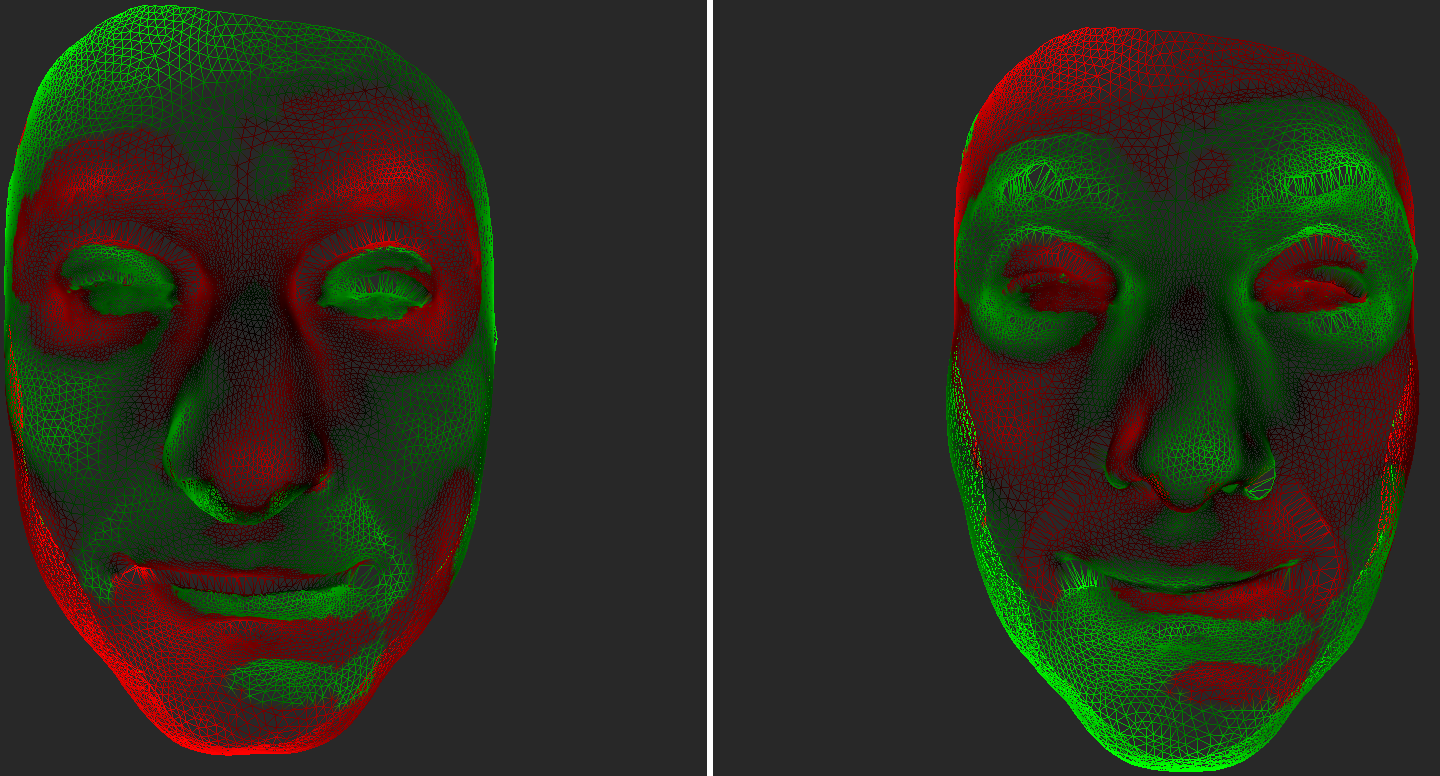
\includegraphics[width=\textwidth]{./screenshots/pair20.PNG}
\caption{}
\label{fig:7-20}
\end{subfigure}
\quad
\begin{subfigure}{0.4\textwidth}
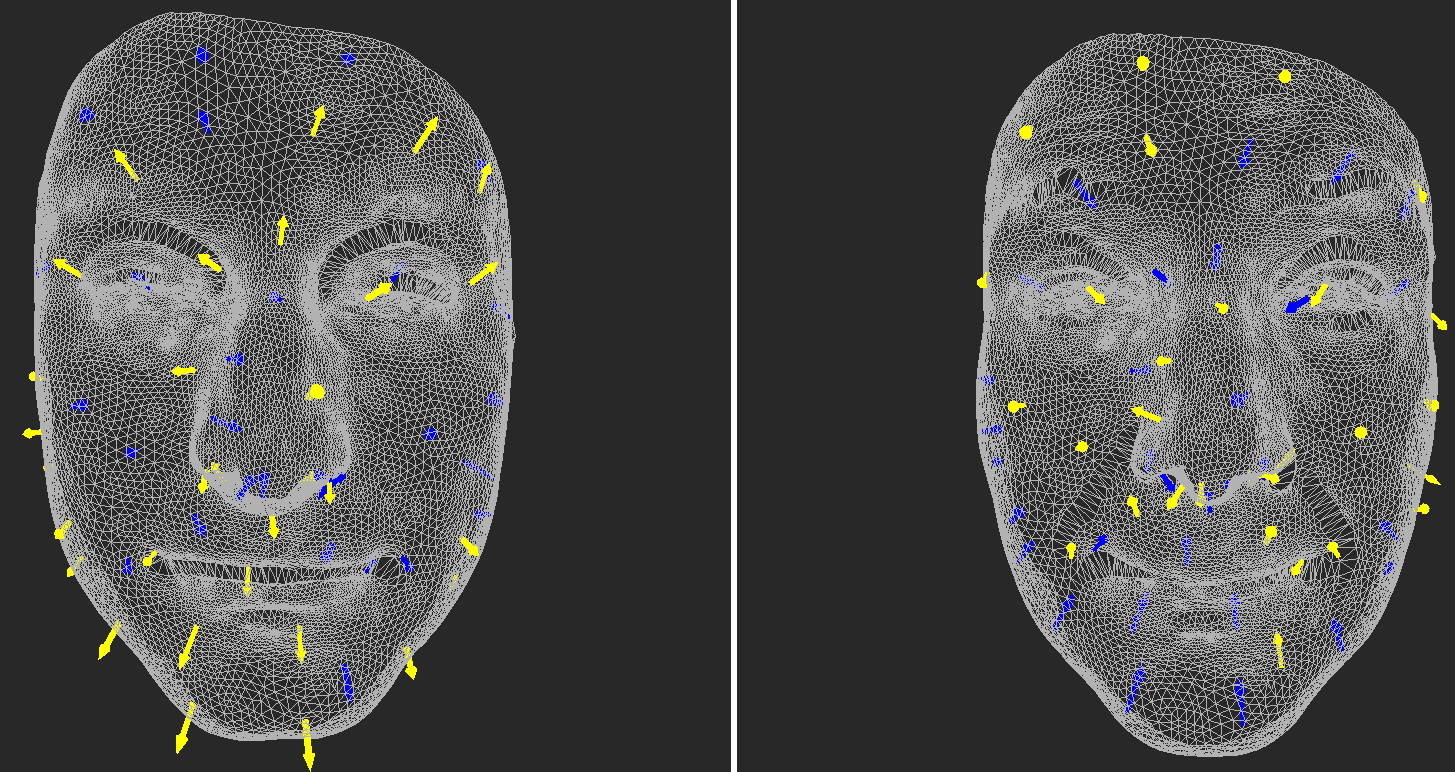
\includegraphics[width=\textwidth]{./screenshots/pair22.PNG}
\caption{}
\label{fig:7-22}
\end{subfigure}

\begin{subfigure}{0.4\textwidth}
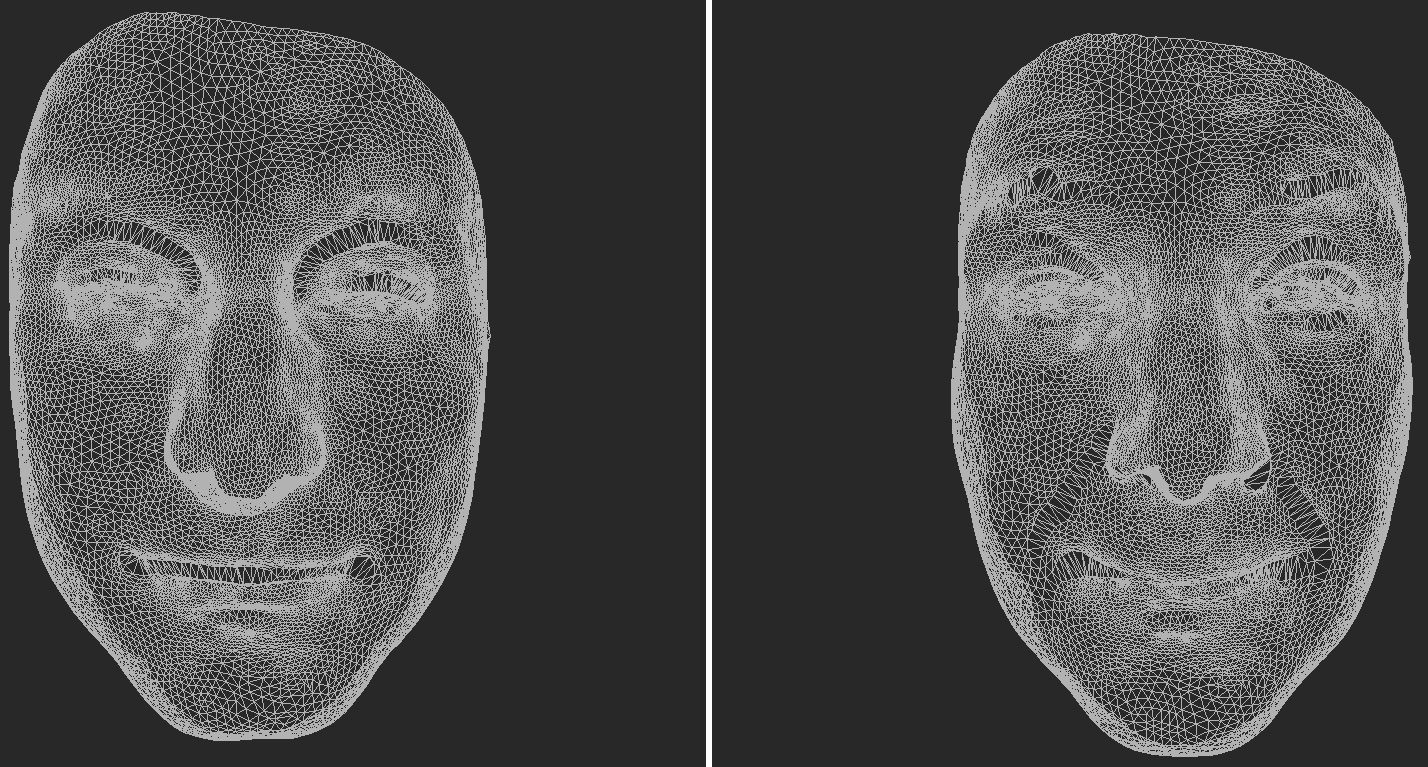
\includegraphics[width=\textwidth]{./screenshots/pair19.PNG}
\caption{}
\label{fig:7-19}
\end{subfigure}
\quad
\begin{subfigure}{0.4\textwidth}
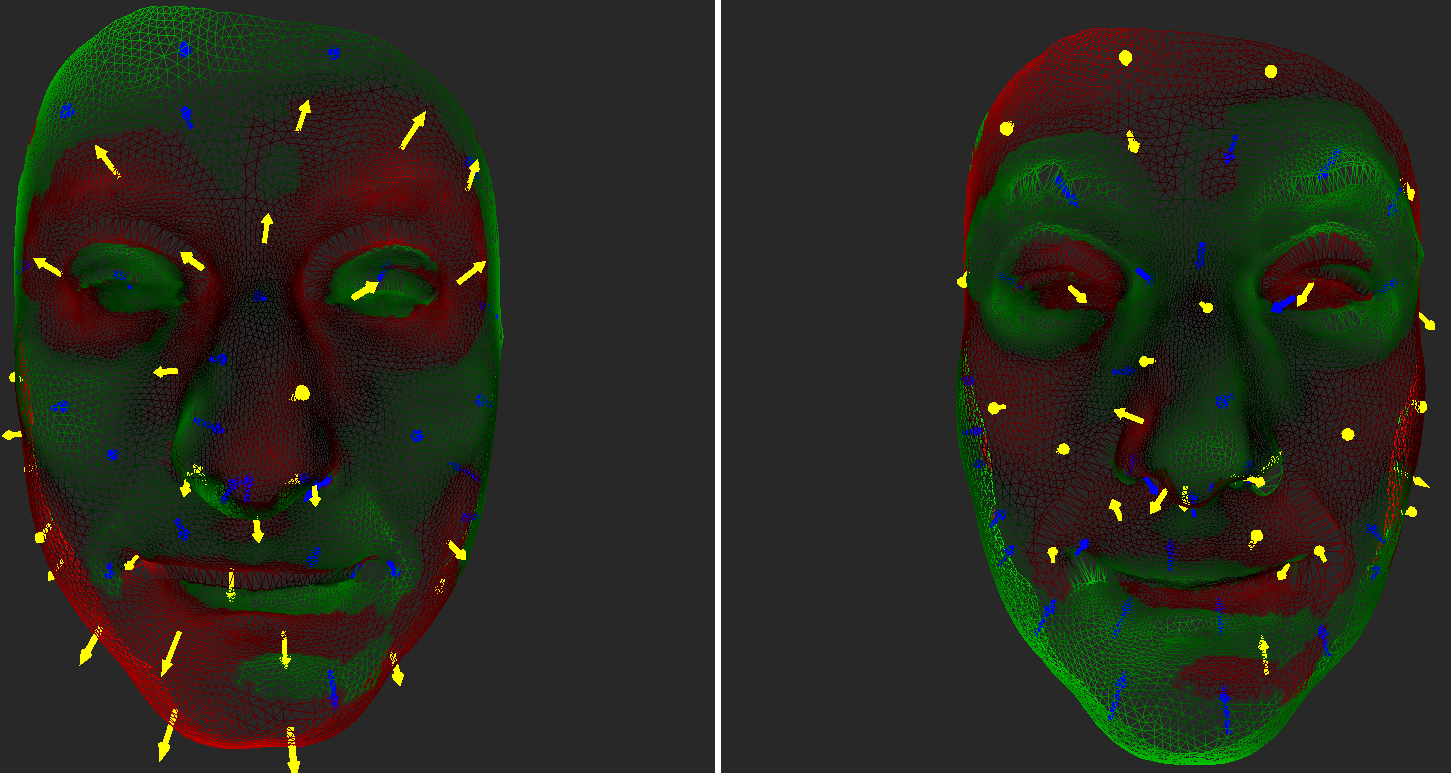
\includegraphics[width=\textwidth]{./screenshots/pair21.PNG}
\caption{}
\label{fig:7-21}
\end{subfigure}
\caption{Visualizations shown to the participants}
\end{figure}
\medskip

\begin{center}
\begin{tabular}{| c | c | c | c | c |}
	\hline
	Visualization & \ref{fig:7-20} & \ref{fig:7-22} & \ref{fig:7-19} & \ref{fig:7-21}\\ \hline
	\(\widehat{t}(p, q_8, V_k)\) & 17.00 & 16.25 & 24.09 & 16.03\\ \hline
	\multicolumn{5}{|c|}{\bf Answers} \\ \hline
	Right & 12 & 8 & 4 & 5\\ \hline
	NotSure & 1 & 0 & 0 & 0\\ \hline
	Left & 0 & 3 & 3 & 1\\ \hline
	{\bf Total} & {\bf 13} & {\bf 11} & {\bf 7} & {\bf 6}\\ \hline
\end{tabular}
\end{center}
\clearpage

\subsection{Question 9}
\label{sec:study-question9}

\begin{center}{\it Where are the two faces the most similar?}\end{center}

\begin{figure}[h]
\centering
\begin{subfigure}{0.4\textwidth}
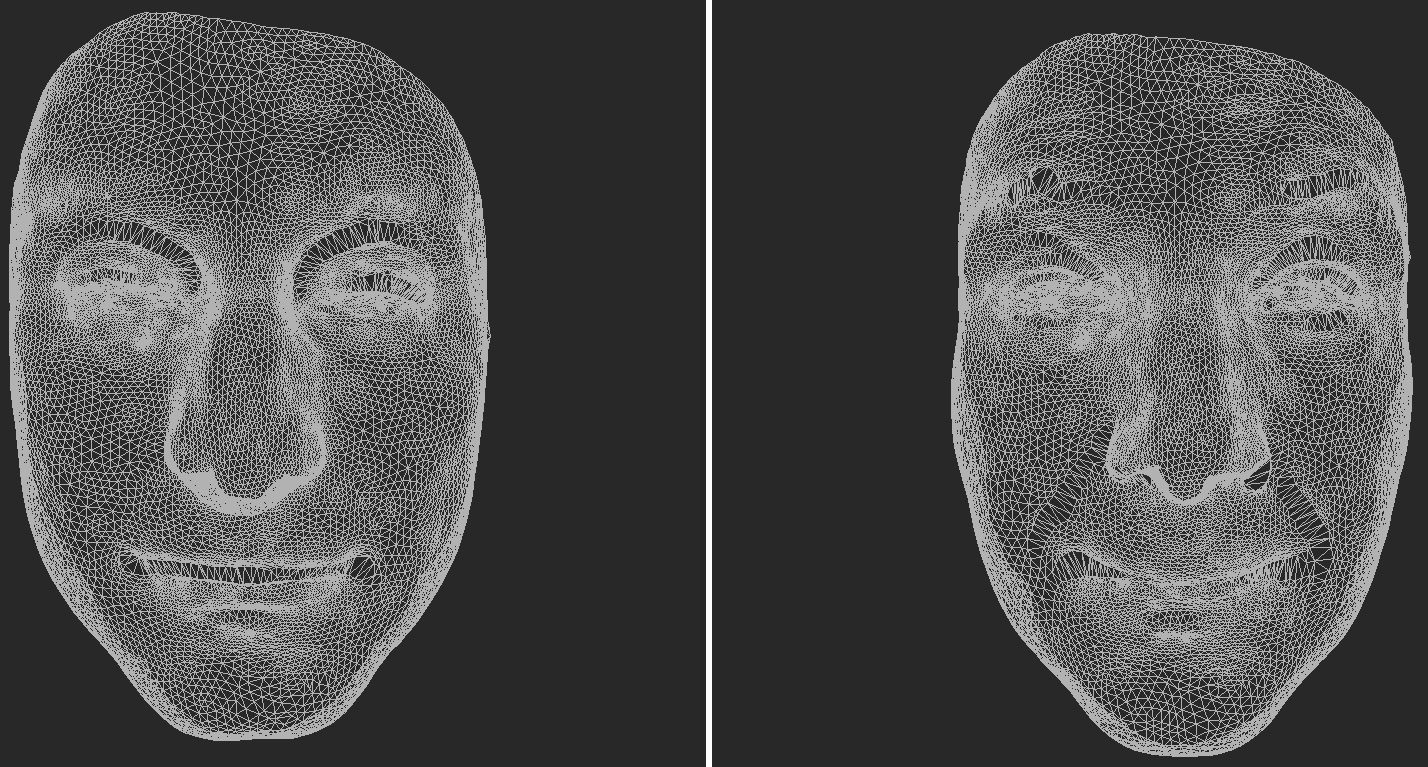
\includegraphics[width=\textwidth]{./screenshots/pair19.PNG}
\caption{}
\label{fig:8-19}
\end{subfigure}
\quad
\begin{subfigure}{0.4\textwidth}
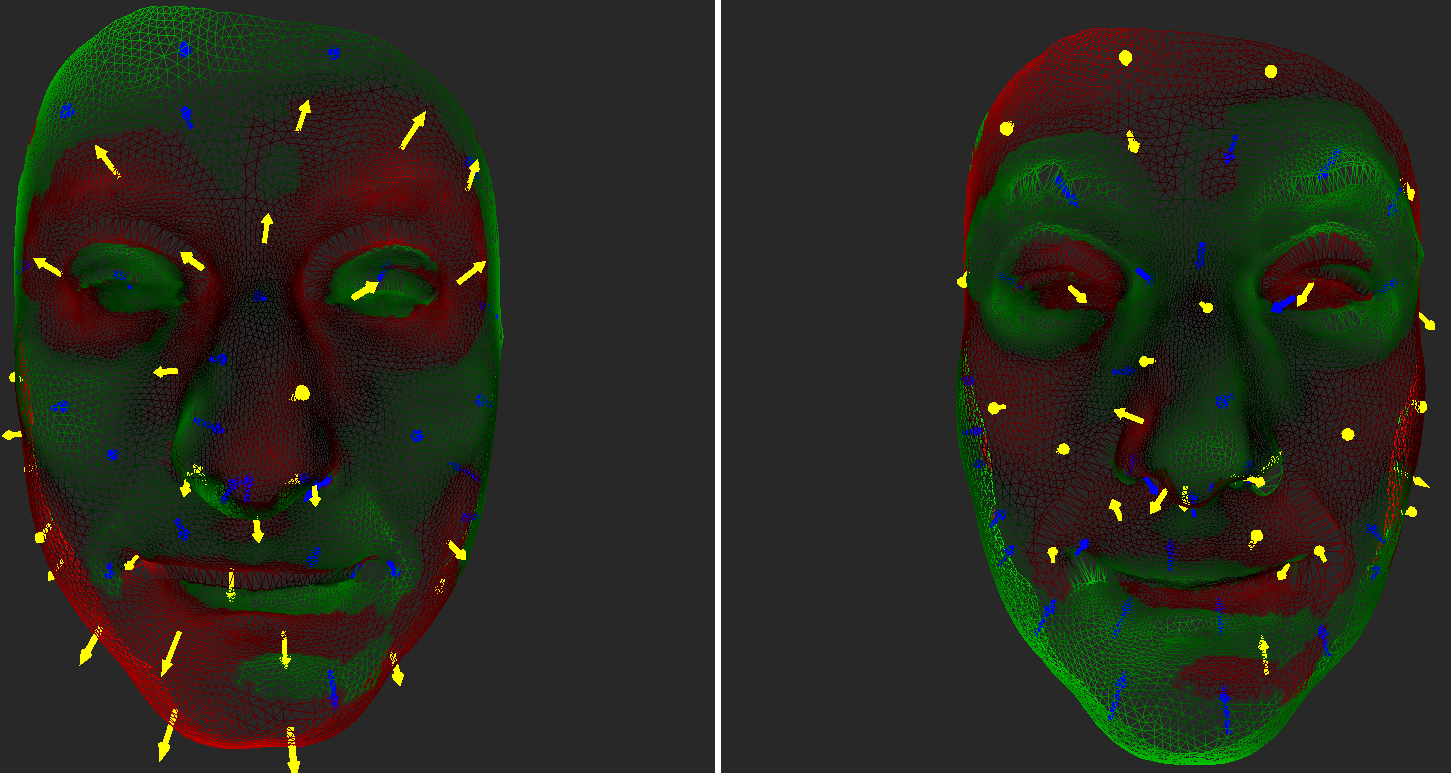
\includegraphics[width=\textwidth]{./screenshots/pair21.PNG}
\caption{}
\label{fig:8-21}
\end{subfigure}

\begin{subfigure}{0.4\textwidth}
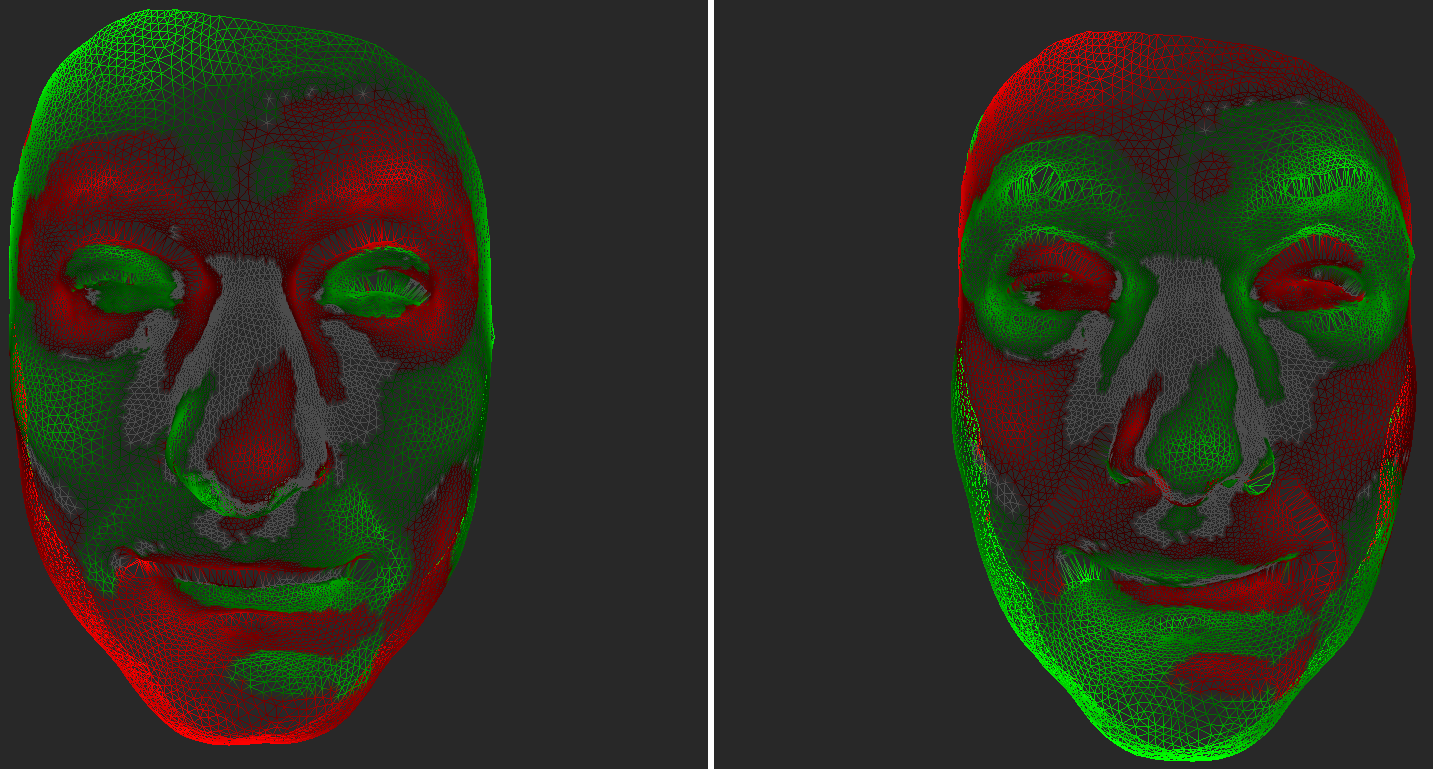
\includegraphics[width=\textwidth]{./screenshots/pair23.PNG}
\caption{}
\label{fig:8-23}
\end{subfigure}
\quad
\begin{subfigure}{0.4\textwidth}
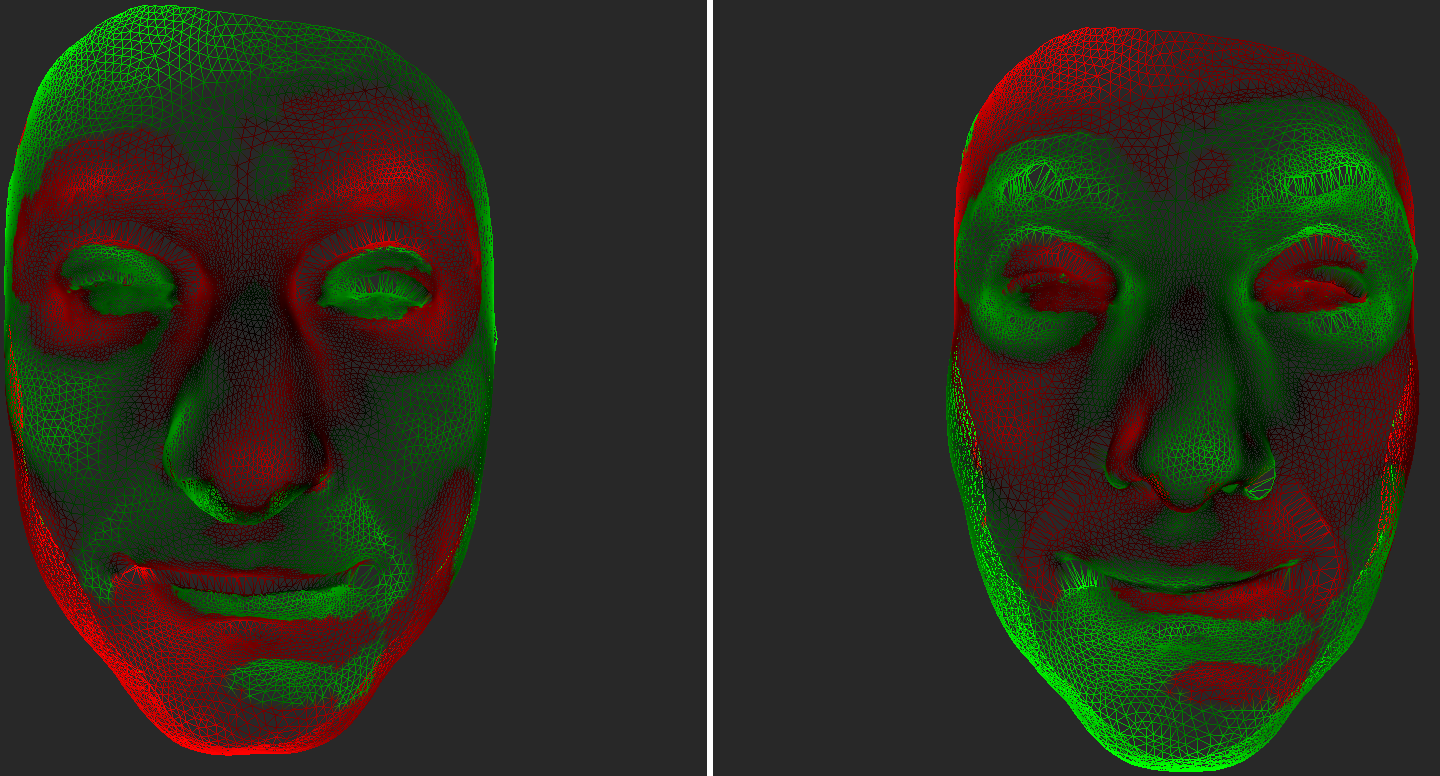
\includegraphics[width=\textwidth]{./screenshots/pair20.PNG}
\caption{}
\label{fig:8-20}
\end{subfigure}
\caption{Visualizations shown to the participants}
\end{figure}
\medskip

\begin{center}
\begin{tabular}{| c | c | c | c | c |}
	\hline
	Visualization & \ref{fig:8-19} & \ref{fig:8-21} & \ref{fig:8-23} & \ref{fig:8-20}\\ \hline
	\(\widehat{t}(p, q_9, V_k)\) & 47.23 & 51.02 & 36.77 & 42.21\\ \hline
	\multicolumn{5}{|c|}{\bf Answers} \\ \hline
	NotSure & 2 & 1 & 1 & 2\\ \hline
	LeftCheek & 2 & 0 & 0 & 0\\ \hline
	Chin & 6 & 0 & 1 & 0\\ \hline
	RightCheek & 3 & 2 & 1 & 2\\ \hline
	Mouth & 0 & 2 & 1 & 0\\ \hline
	Nose & 0 & 5 & 3 & 1\\ \hline
	Forehead & 0 & 1 & 0 & 1\\ \hline
	{\bf Total} & {\bf 13} & {\bf 11} & {\bf 7} & {\bf 6}\\ \hline
\end{tabular}
\end{center}
\clearpage

\subsection{Question 10}
\label{sec:study-question10}

\begin{center}{\it When examining the differences moving from the left face to the right face, what is their main direction overall?}\end{center}

\begin{figure}[h]
\centering
\begin{subfigure}{0.4\textwidth}
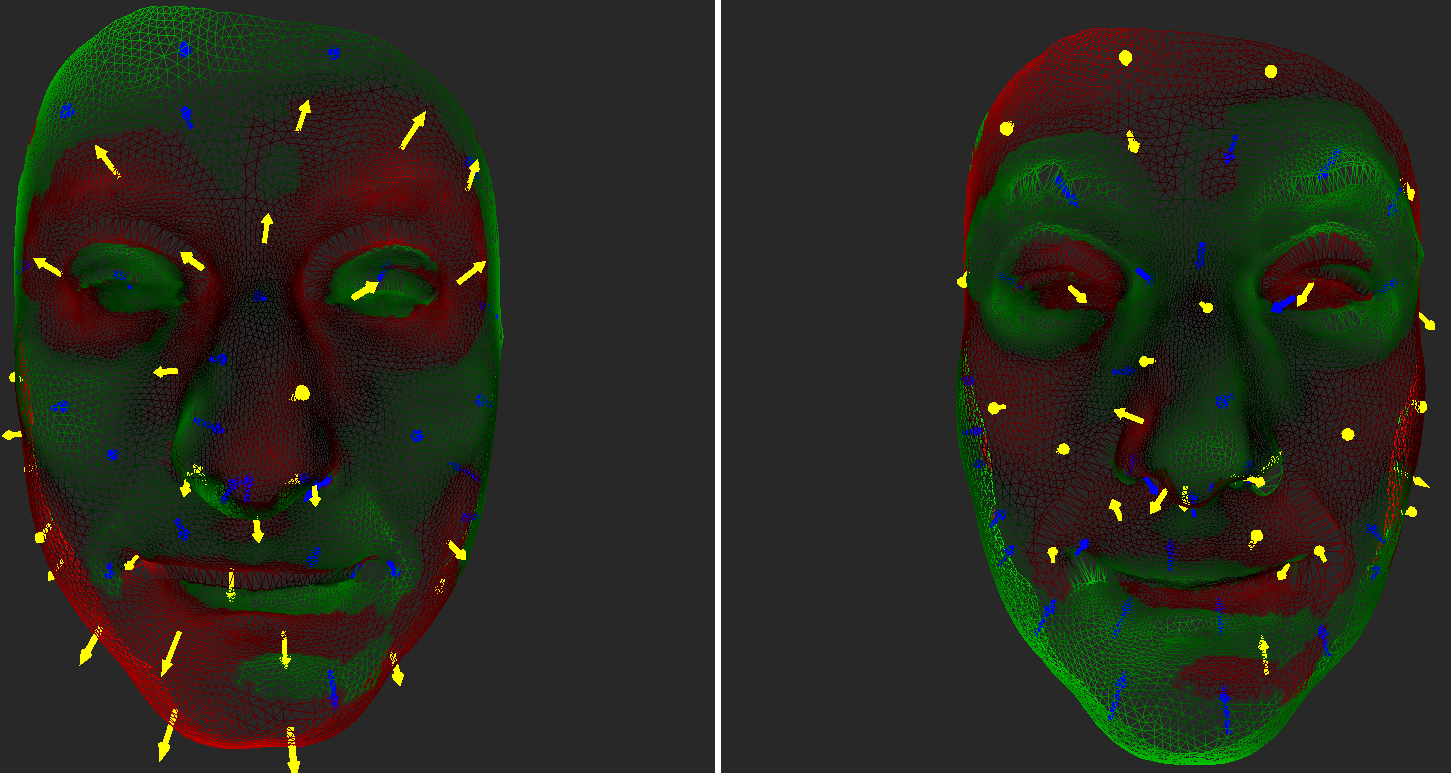
\includegraphics[width=\textwidth]{./screenshots/pair21.PNG}
\caption{}
\label{fig:9-21}
\end{subfigure}
\quad
\begin{subfigure}{0.4\textwidth}
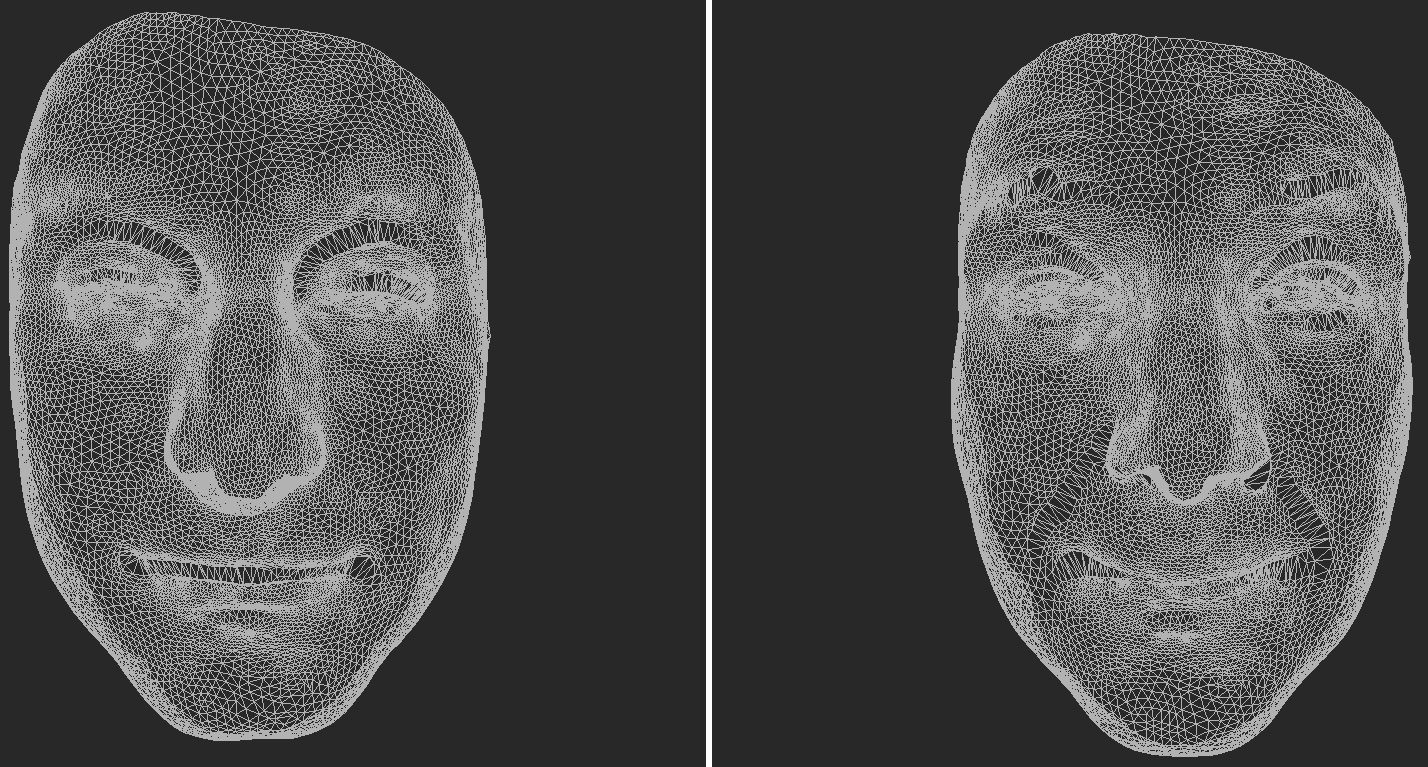
\includegraphics[width=\textwidth]{./screenshots/pair19.PNG}
\caption{}
\label{fig:9-19}
\end{subfigure}

\begin{subfigure}{0.4\textwidth}
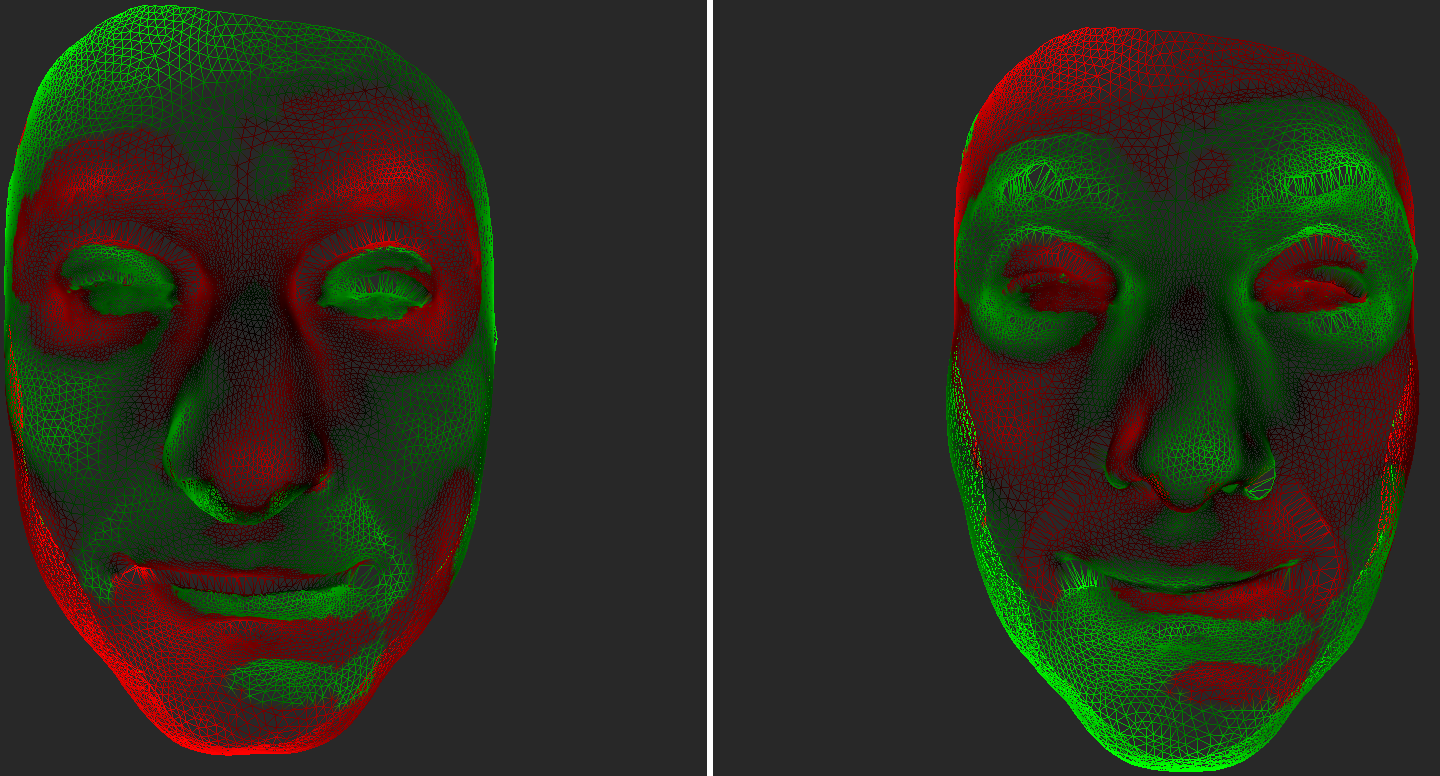
\includegraphics[width=\textwidth]{./screenshots/pair20.PNG}
\caption{}
\label{fig:9-20}
\end{subfigure}
\quad
\begin{subfigure}{0.4\textwidth}
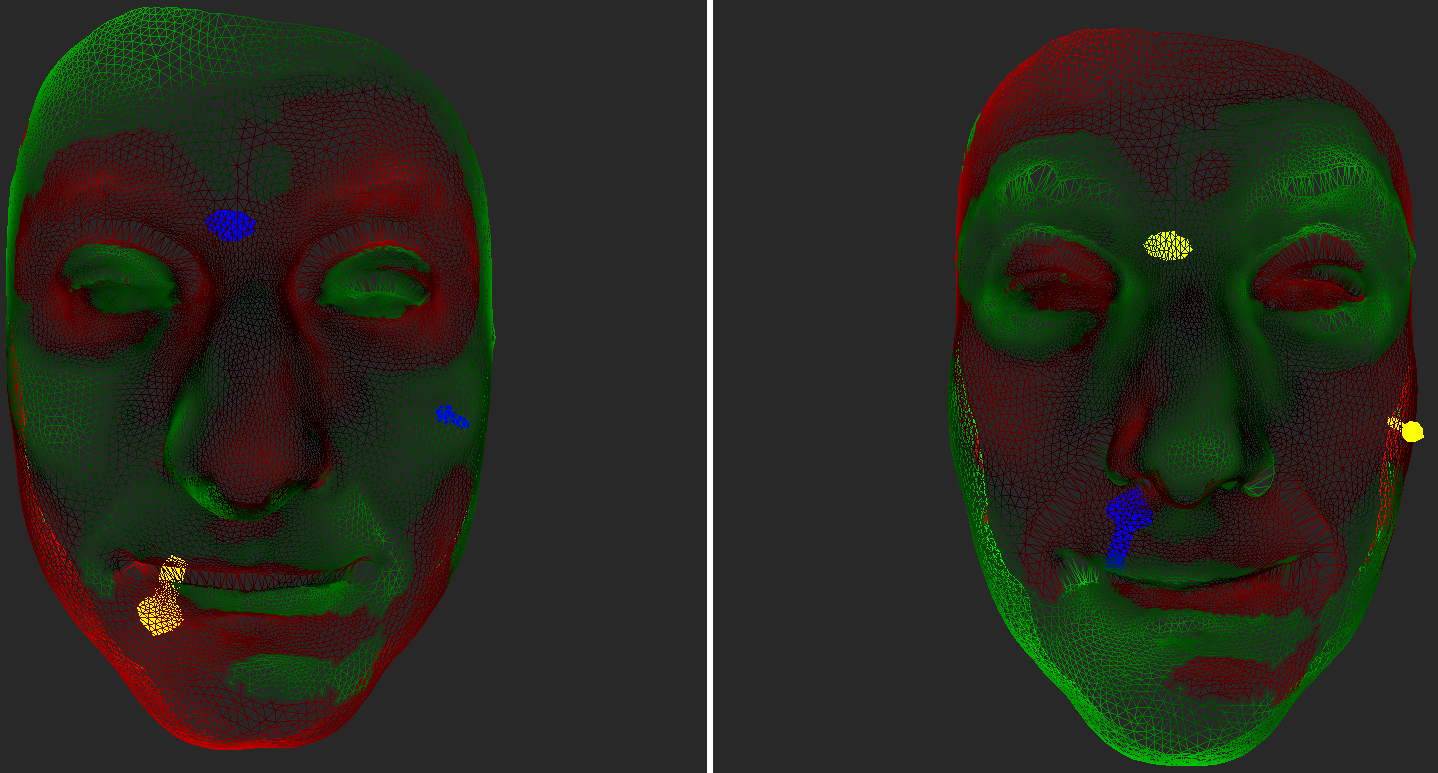
\includegraphics[width=\textwidth]{./screenshots/pair24.PNG}
\caption{}
\label{fig:9-24}
\end{subfigure}
\caption{Visualizations shown to the participants}
\end{figure}
\medskip

\begin{center}
\begin{tabular}{| c | c | c | c | c |}
	\hline
	Visualization & \ref{fig:9-21} & \ref{fig:9-19} & \ref{fig:9-20} & \ref{fig:9-24}\\ \hline
	\(\widehat{t}(p, q_10, V_k)\) & 50.42 & 33.90 & 48.06 & 53.28\\ \hline
	\multicolumn{5}{|c|}{\bf Answers} \\ \hline
	NotSure & 4 & 2 & 2 & 1\\ \hline
	Down & 3 & 1 & 1 & 2\\ \hline
	In & 2 & 1 & 1 & 0\\ \hline
	Out & 3 & 4 & 2 & 0\\ \hline
	Up & 1 & 2 & 0 & 2\\ \hline
	Left & 0 & 1 & 0 & 0\\ \hline
	Right & 0 & 0 & 1 & 1\\ \hline
	{\bf Total} & {\bf 13} & {\bf 11} & {\bf 7} & {\bf 6}\\ \hline
\end{tabular}
\end{center}
\clearpage

